% !TeX spellcheck = en_US
\documentclass[a4paper]{report}
\usepackage[T1]{fontenc}
\usepackage[utf8]{inputenc}
\usepackage[english]{babel}
\usepackage{geometry}
\usepackage{graphicx}
\usepackage{subfig}
\usepackage{lipsum}
\usepackage{verbatim}
\usepackage[table,xcdraw]{xcolor}
 \geometry{a4paper,top=2.5cm,bottom=2.5cm,left=3cm,right=3cm,%
	heightrounded,bindingoffset=5mm}

\usepackage{color}
\usepackage{listings}
\usepackage{xcolor}

\colorlet{punct}{red!60!black}
\definecolor{background}{HTML}{EEEEEE}
\definecolor{delim}{RGB}{20,105,176}
\colorlet{numb}{magenta!60!black}


\lstdefinelanguage{json}{
	basicstyle=\normalfont\ttfamily,
	numbers=left,
	numberstyle=\scriptsize,
	stepnumber=1,
	numbersep=8pt,
	showstringspaces=false,
	breaklines=true,
	frame=lines,
	backgroundcolor=\color{background},
	literate=
	*{:}{{{\color{punct}{:}}}}{1}
	{,}{{{\color{punct}{,}}}}{1}
	{\{}{{{\color{delim}{\{}}}}{1}
	{\}}{{{\color{delim}{\}}}}}{1}
	{[}{{{\color{delim}{[}}}}{1}
	{]}{{{\color{delim}{]}}}}{1},
}



\lstdefinelanguage{code}{ 
	backgroundcolor=\color{white},   % choose the background color; you must add \usepackage{color} or \usepackage{xcolor}; should come as last argument
	basicstyle=\footnotesize,        % the size of the fonts that are used for the code
	breakatwhitespace=false,         % sets if automatic breaks should only happen at whitespace
	breaklines=true,                 % sets automatic line breaking
	captionpos=b,                    % sets the caption-position to bottom
	commentstyle=\color{black},    % comment style
	deletekeywords={...},            % if you want to delete keywords from the given language
	escapeinside={\%*}{*)},          % if you want to add LaTeX within your code
	extendedchars=true,              % lets you use non-ASCII characters; for 8-bits encodings only, does not work with UTF-8
	firstnumber=1,                % start line enumeration with line 1
	frame=single,	                   % adds a frame around the code
	keepspaces=true,                 % keeps spaces in text, useful for keeping indentation of code (possibly needs columns=flexible)
	keywordstyle=\color{black},       % keyword style
	language=Octave,                 % the language of the code
	morekeywords={*,...},            % if you want to add more keywords to the set
	numbers=left,                    % where to put the line-numbers; possible values are (none, left, right)
	numbersep=5pt,                   % how far the line-numbers are from the code
	numberstyle=\tiny\color{black}, % the style that is used for the line-numbers
	rulecolor=\color{black},         % if not set, the frame-color may be changed on line-breaks within not-black text (e.g. comments (green here))
	showspaces=false,                % show spaces everywhere adding particular underscores; it overrides 'showstringspaces'
	showstringspaces=false,          % underline spaces within strings only
	showtabs=false,                  % show tabs within strings adding particular underscores
	stepnumber=1,                    % the step between two line-numbers. If it's 1, each line will be numbered
	stringstyle=\color{black},     % string literal style
	tabsize=2,	                   % sets default tabsize to 2 spaces
		literate=
	*{:}{{{\color{black}{:}}}}{1}
	{,}{{{\color{black}{,}}}}{1}
	{\{}{{{\color{black}{\{}}}}{1}
	{\}}{{{\color{black}{\}}}}}{1}
	{[}{{{\color{black}{[}}}}{1}
	{]}{{{\color{black}{]}}}}{1},
}


\lstset{ %
	language=C++,                % choose the language of the code
	basicstyle=\footnotesize,       % the size of the fonts that are used for the code
	numbers=left,                   % where to put the line-numbers
	numberstyle=\footnotesize,      % the size of the fonts that are used for the line-numbers
	stepnumber=1,                   % the step between two line-numbers. If it is 1 each line will be numbered
	numbersep=5pt,                  % how far the line-numbers are from the code
	backgroundcolor=\color{white},  % choose the background color. You must add \usepackage{color}
	showspaces=false,               % show spaces adding particular underscores
	showstringspaces=false,         % underline spaces within strings
	showtabs=false,                 % show tabs within strings adding particular underscores
	frame=single,           % adds a frame around the code
	tabsize=2,          % sets default tabsize to 2 spaces
	captionpos=b,           % sets the caption-position to bottom
	breaklines=true,        % sets automatic line breaking
	breakatwhitespace=false,    % sets if automatic breaks should only happen at whitespace
	escapeinside={\%*}{*)}          % if you want to add a comment within your code
}



\newcommand{\HRule}{\rule{\linewidth}{0.5mm}}

\begin{document}
\begin{titlepage}
	\begin{center}
		
		% Top 
		
\includegraphics[width=0.45\textwidth]{img/unipi.png}~\\[2.5cm]
		
		
		% Title
		\HRule \\[0.4cm]
		{ \LARGE 
			\textbf{JustRecipe}\\[0.4cm]
			\emph{Group Project for Large Scale and Multi-Structured Databases}\\[0.4cm]
		}
		\HRule \\[1.5cm]
		
		
		
		% Author
		{ \large
			Francesco Campilongo \\[0.1cm]
			Daniele Cioffo \\[0.1cm]
			Francesco Iemma \\[0.1cm]
		}
		
		\vfill

		%\textsc{\large Department of Electrical Engineering,\\Computer Engineering \& Informatics}\\[0.4cm]
		
		
		% Bottom
		{\large Academic Year 2020/21}
		
	\end{center}
\end{titlepage}


\tableofcontents

\chapter*{Introduction}
In the social network era the large scale databases topic is very relevant. The handling of big data such as informations of users and moreover is a critical asset of our society. In fact, from the viewpoint of the security is very important to handle in the correct way this very huge amount of data because, otherwise, it is possible to have leak of critical information that cause critical issues about users privacy.

\noindent Another problem caused from large amount of data created from the applications used every day from all of us, is the following: \emph{How we can manage this data?}.

\noindent Nowadays we have a lot of tools to do this, the most famous, and maybe the most used, is for sure MongoDB. It allows us to handle a huge amount of data without critical issues and maintaining good performance. Another well-known tool is Neo4J (and so Graph DB) that is in charge of handle the social part of the application, in fact the graph is indeed a network, and so this is the best way to represents a social network where the interactions between users are fundamental and very widespread.

\noindent Our aim is to design and implement a modern application which can handle a huge amount of data maintaining good performance and implementing a social network side in order to exploit the desire for social relations of our society.



\chapter{Dataset}
In this first chapter of this document we will talk about searching for the initial dataset.

\noindent As specified in the project documentation, the dataset had to be at least 50MB large, and this quantity could not be generated directly within the application. So we did an initial search, finding two datasets, which were generated by their authors by performing the scraping on the sites \emph{www.FoodNetwork.com} and \emph{www.Epicurios.com}. The second dataset was more complete (more nutritional values), so it was used as the main dataset. The other dataset was used to complement the other, reaching a total of  67.8 MB, with 45349 recipes.

\noindent To correctly extract the data present in the two datasets we wrote a program in Java, called \emph{RecipeReade}r, thanks to which we adapted the two different formats and removed the duplicates (recipes with the same title that were present in both datasets).
To implement this program we used the GSon library and the Jackson library.

\noindent The variety property is ensured by using two different sources. The velocity / variability properties are ensured because comments and recipes are eliminated and added inside the application, indeed this data may lose importance after a certain time interval since new data quickly arrives.

\chapter{Design}
\section{Introduction To The Application}
The topic of cuisine is extensively widespread in our society. In fact we can think at the success achieved by tv shows related to cooking in the last years and also at the fact that a lot of chefs are becoming superstars.
Then there is another important factor: the coronavirus outbreak.

\noindent With the coronavirus outbreak a lot of people became cuisine lovers, in fact at the first moments of the pandemia several ingredients as flour and yeast were very hard to find, because people were confined in their home and so they had more free time.

\noindent But this topic is not a recente one. The first recipe book dates back to eigth century B.C. and it is the so-called \emph{Eraclio} (by the name of the city in which he was found). Then also an important latin writer, Apicio, wrote one of the most important recipe books of the roman era: \emph{De Re Coquinaria} which dates back to the first century B.C..
 
\noindent So the topic of cuisine is inherent to human nature, because the necessity of eating is a basic need.
Furthermore, everyone has experimented the infamous question: “What will I eat this evening?”. JustRecipe has the aim of answer to this question, it has the aim of helping university student or workers to retrieve and to do fast and simple recipes.

\noindent So this application is basically a recipe book but it is also more than this.

\noindent JustRecipe is also a social network which allow people to enjoy, to ex-change ideas about cooking, to feel less lonely in this hard period.

\section{Requirements}
\subsection{Main Actors}
The main actors of the application are four:
\begin{itemize}
	\item Unregistered User
	
	\noindent He is the user which opens the application for the first time, in order to access he must sign-up.
	
	\item User
	
	\noindent He is the normal user (the registered one).
	
	\item Moderator
	
	\noindent He is in charge of controlling the comments and eventually delete the ones which contain abuses.
	
	\item Administrator
	
	\noindent He is the most powerful actor, he can delete users and recipes and he is also in charge of elect moderators and others administrators. When a user becomes administrator, this privilege cannot be revoked.
\end{itemize}

\noindent Each actor can do all the features of the previous ones in the list.

\subsection{Functional Requirements}
\subsubsection{Features offered to the Unregistered User}
\begin{itemize}
	\item  Registration
	
	\noindent In order to access the application an user must sign-up. Otherwise he is not allowed to access and to use all the functionalities.
\end{itemize}
\subsubsection{Features offered to the Registered User}
\begin{itemize}
	\item Login/Logout
	
	\noindent The only way to access the application, as we said previously, is to sign-up and login. At the end the user can logout and close the session.
	
	\item Search a recipe
	
	\noindent It's possible to search a recipe searching for the title and for categories.
	
	\item Browse suggested recipes
	
	\noindent The suggestions will be offered in a proper section, they are done considering the relationships between the user logged, the users followed by the user logged and so on so forth.
	
	\item Browse recipes of following users
	
	\noindent In a proper section (i.e. the Homepage) the user can browse the recipes of the following users. Indeed he can see only a snapshot of the recipes. If he wants a more in-depth view, he can click on it and see the recipe page in which he is able to see all the recipe details. 
	
	\item Add a recipe
	
	\noindent The user can insert a new recipe.
	
	\item Edit own recipes
	
	\noindent The user can edit the recipes previously added by himself.
	
	\item Comment recipes
	
	\noindent
	Every user can make a comment about recipes
	
	\item Follow another user
	
	\noindent The most important feature of each social network: the users can follow each others. 
	
	
	\item Like a recipe
	
	\noindent In order to evaluate a recipe each user can like it.
\end{itemize}

\subsubsection{Features offered to the Moderator}
\begin{itemize}
	\item Delete comments
	
	\noindent The moderator is in charge of delete comments which contain racist abuse, crude terms and so on so forth.
\end{itemize}

\subsubsection{Features offered to the Administrator}
\begin{itemize}
	\item Delete users
	
	\noindent The admin can delete the users which don't respect the application guidelines.
	
	\item Delete recipes
	
	\noindent The admin can delete recipes not correctly inserted
	
	\item Elect/Dismiss moderators
	
	\noindent In order to handle better the application, the admin can elect some users as moderators.
	
	\item Elect administrators
	
	\noindent The admin can elect other administrators.
\end{itemize}
\subsection{Non-Functional Requirements}
The non-functional requirements of the applications are described in the following lists:
\begin{itemize}
	\item \emph{Usability}: The application must be user-friendly so a GUI is adopted. A low response time is necessary in order to avoid too long waits for the user.
	\item \emph{Data Availability}: For modern shared-data systems and for a social network application, the most crucial requirement is that the data must be always available as the service too.
	\item \emph{Tolerance to single point of failure}: If a server crashes another one is available, this is ensured by the use of replicas.
	\item \emph{Data Consistency}: The operations must be monotonic and so all the users must see the last version of the data and the update operations must be performed in the same order in which they are issued.

	\item \emph{Reliability}: The application must work without crashes and so it must handle exceptions if they occur.
	
	\item \emph{Flexibility}: Due to the fact that the recipes attribute are not all mandatory, the data must be handled in a flexible way.  
\end{itemize}
\newpage
\subsection{Actors and Use Cases}
The use case diagram of the application is described in the figure 2.1

\begin{figure}[htpb]
	\centering
	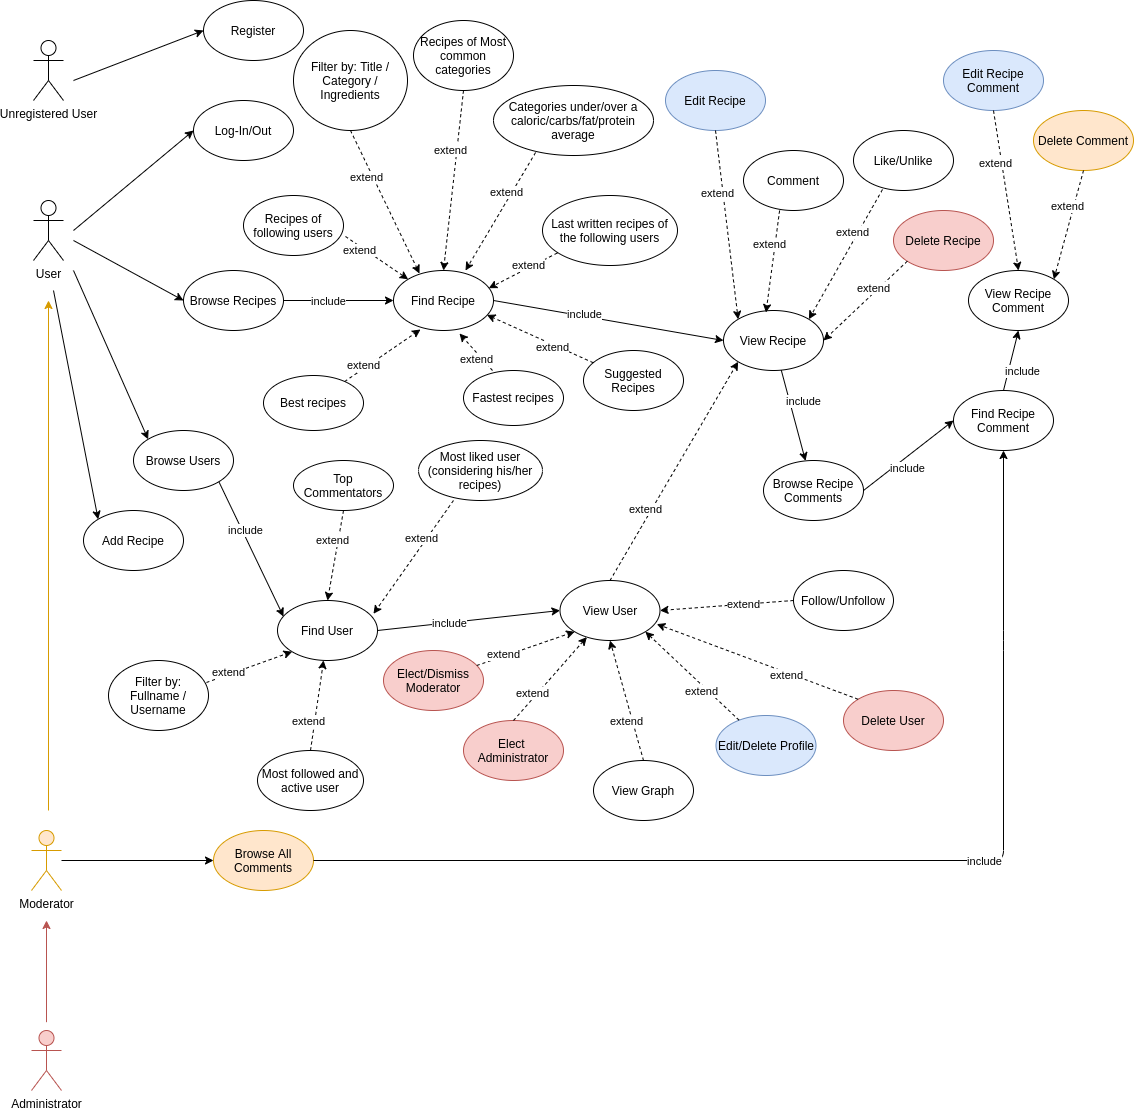
\includegraphics[scale=0.4]{img/UseCaseDiagram.png}
	\caption{Use Case Diagram}
\end{figure}

\noindent Some observations on the diagram are necessary:
\begin{itemize}
	\item The circles in \underline{blue} are the ones which described actions available only for the owner of the object on which the actions are applied.
	
	\noindent So, in detail, this means that a \textbf{User} can edit/delete a profile if and only if he owns this profile. Then he can edit a recipe and/or a comment if and only if he adds that recipe or that comment.
	
	\item When we are seeing the recipe detail we can go on the user that have been added that recipe. So the extend relation between \emph{View Recipe} and \emph{View User} means this.
	
	\item The action \emph{Browse Recipes of following users} is available only if the \textbf{User} follows at least one user. Otherwise he can start to follow users and only after this he can see suggested recipes (\emph{Browse Suggested Recipes}). In this case, due to the fact that the user follows nobody, he will see the most famous recipes in general because it's impossible to suggest specific recipes due to the fact that he has no following and no likes or comments. 
	
	\item The actions in \underline{red} are the ones that can be performed only by the \textbf{Administrator}
	
	\item The actions in \underline{orange} are the ones that can be performed only by the \textbf{Moderators}
\end{itemize}


\section{UML Class Diagram}
Let analyze the UML Class Diagram. There are three main entities: User, Comment, Recipe.

\noindent It's important to point out that the \textbf{User} of the Use Case Diagram is here the so-called \emph{Registered User} and the \emph{User} of this diagram is the generic user. Then we underline the fact that, in order to represent the three actors of the use case diagram, a generalization is needed.
 
\begin{figure}[htpb]
	\centering
	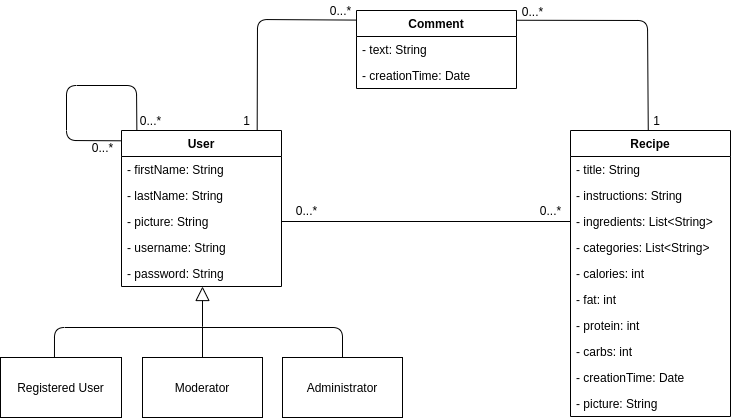
\includegraphics[scale=0.5]{img/ClassDiagram_generaliz.png}
	\caption{UML Analysis Classes Diagram with generalization unsolved}
\end{figure}

\noindent Observing the figure 2.2 it's possible to understand that we can resolve the generalization putting an attribute in the entity \emph{User}. It is an integer and we call it \emph{role}: if it's a \emph{Normal User} role is 0; if \emph{Moderator} then 1; if \emph{Administrator} then 2.

\begin{figure}[htpb]
	\centering
	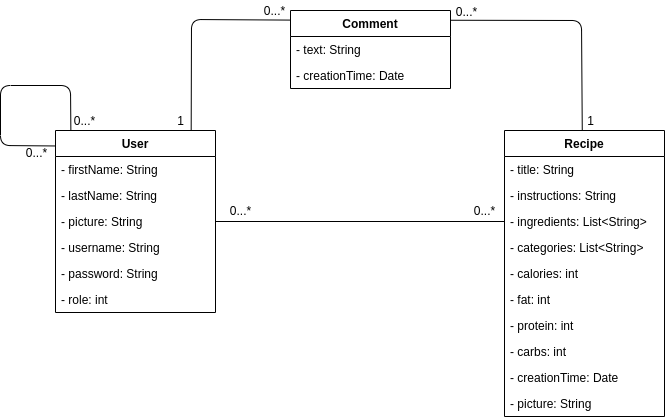
\includegraphics[scale=0.5]{img/ClassDiagram.png}
	\caption{UML Analysis Classes Diagram}
\end{figure}

Let analyze the attributes for each class in the following tables.

\begin{table}[htpb]
\caption{Classes definitions}
\centering 
\begin{tabular}{|l|l|}
\hline
\rowcolor[HTML]{000000} 
{\color[HTML]{FFFFFF} Class} & {\color[HTML]{FFFFFF} Description}                                            \\ \hline
Registered User              & A standard user (registered one) who can only perform basic operations        \\ \hline
Moderator                    & User who can also check comments and decide to delete them                    \\ \hline
Administrator                & Most powerful user, he can also delete users and recipes, and elect moderator \\ \hline
Comment                      & Comment posted by a user                                                      \\ \hline
Recipe                       & Recipe added by one user                                                      \\ \hline
\end{tabular}
\end{table}

\begin{table}[htpb]
\caption{Classes attributes - User}
\centering 
\begin{tabular}{|l|l|l|}
\hline
\rowcolor[HTML]{000000} 
{\color[HTML]{FFFFFF} Attribute} & {\color[HTML]{FFFFFF} Type} & {\color[HTML]{FFFFFF} Description}                                \\ \hline
firstName                        & String                      & First name of the user                                            \\ \hline
lastName                         & String                      & Last name of the user                                             \\ \hline
picture                          & String                      & URL of the picture                                                \\ \hline
username                         & String                      & Username of the user (identifier)                                 \\ \hline
password                         & String                      & Password chosen by the user, used for the login phase             \\ \hline
role                             & int                         & Role of the user (0: Normal User, 1: Moderator, 2: Administrator) \\ \hline
\end{tabular}
\end{table}


\begin{table}[htpb]
\caption{Classes attributes - Comment}
\centering
\begin{tabular}{|l|l|l|}
\hline
\rowcolor[HTML]{000000} 
{\color[HTML]{FFFFFF} Attribute} & {\color[HTML]{FFFFFF} Type} & {\color[HTML]{FFFFFF} Description} \\ \hline
text                             & String                      & Plain text of the comment          \\ \hline
creationTime                     & Date                        & Creation timestamp of the comment  \\ \hline
\end{tabular}
\end{table}

\begin{table}[]
	\caption{Classes attributes - Recipe}
	\centering
	\begin{tabular}{|l|l|l|}
		\hline
		\rowcolor[HTML]{000000} 
		{\color[HTML]{FFFFFF} Attribute} & {\color[HTML]{FFFFFF} Type}         & {\color[HTML]{FFFFFF} Description}           \\ \hline
		title                            & String                              & Title of the recipe (identifier)             \\ \hline
		instructions                     & String                              & Operation to be performed to make the recipe \\ \hline
		ingredients                      & List\textless{}String\textgreater{} & Ingredients to be used in the recipe         \\ \hline
		categories                       & List\textless{}String\textgreater{} & Categories to which the recipe belongs       \\ \hline
		calories                         & int                                 & Calories contained in the recipe             \\ \hline
		fat                              & int                                 & Fat contained in the recipe                  \\ \hline
		protein                          & int                                 & Protein contained in the recipe              \\ \hline
		carbs                            & int                                 & Carbs contained in the recipe                \\ \hline
		creationTime                     & Date                                & Creation timestamp of the recipe             \\ \hline
		picture                          & String                              & URL of the recipe picture                    \\ \hline
	\end{tabular}
\end{table}


\newpage

\newpage

\section{Data Model}
In this section we will discuss about the design choises performed in terms of data model in order to handle in the better way our dataset.
\subsection{DocumentDB}
The document database is used in order to deal with a very large amount of data in an easy and fast way. So due to the fact that our dataset is very large this is the best design choice to achieve the \emph{usability} requirement, in particular for what is related to the latency. Moreover, we use a DocumentDB in order to respect the \emph{flexibility} requirement, in fact it is schema-less and this allow us to maintain heterogeneous recipes in our database. For instance the user can insert a recipe without some attributes (carbs and fat for example) and we have no issues due to the schema-less property of DocumentDB. Furthermore this is very important for what concern the comments: in fact comments are embedded in the recipe document and the schema-less approach allow us to add comment in a flexible way and to have recipes without comments.
So, to summarize, we use only one collection, \emph{recipes}, in which every document is a recipe that contains also the comments. So this is how we decided to implements the \emph{one-to-many} relationship between \emph{Recipe} and \emph{Comment}.

\noindent This is an example of one Recipe that contains all the value (this is not mandatory, like we said before):

\lstset{ language=json}
\begin{lstlisting}
{
	"_id":
			{"$oid": "5fdb5fd86796ee4e73ef5b84"},
	"title": 
			"Lentil, Apple, and Turkey Wrap ",
	"instructions": 
			"1. Place the stock, lentils, celery, carrot, thyme, and
			salt in a medium saucepan and bring to a boil. Reduce heat
			to low and simmer until the lentils are tender, about 30
			minutes, depending on the lentils. (If they begin to
			dry out, add water as needed)..." ,
	"ingredients":
			["4 cups low-sodium vegetable or chicken stock", "1 cup dried brown lentils", ...],
	"categories":
			["Sandwich", "Bean", "Fruit", "Tomato", "turkey", ...],
	"calories":
			426,
	"fat":
			7,
	"protein":
			30,
	"carbs":
			20,
	"creationTime":
			{
				"$date": "2020-12-17T13:40:40.658Z"
			},
	"authorUsername":
			"oscar.evans",
	"picture":
			"https://assets.epicurious.com/photos/551b0595e7851a541a30b23f/master/pass/239173_lentil-apple-and-turkey-wrap_6x4.jpg",
	"comments":
			[
				{
					"authorUsername": "oliver.smith",
					"text": "Very good!!!",
					"creationTime":
					{
						"$date": "2020-12-17T13:50:40.658Z"
					}
				},
				{
					"authorUsername": "jessica.evans",
					"text": "Fantastic",
					"creationTime":
					{
						"$date": "2020-12-17T13:52:40.658Z"
					}
				},....
			]
}
\end{lstlisting}  
\subsection{GraphDB}
The Graph database is the one that handles the social part of the application. Thanks to it we are able to analyze the relationships among users and their recipes.

\noindent We have two type of nodes within the database:
\begin{itemize}
	\item \textbf{User}: it is the node that represents the user inside the graph. Its attribute are: \emph{firstName}, \emph{lastName}, \emph{username}, \emph{password}, \emph{picture}\footnote{Only the URL of the picture is saved in this field, otherwise the size of this attribute would be too large}, \emph{role}\footnote{0 for the normal user, 1 for moderator and 2 for the administrator}.
	
	\item \textbf{Recipe}: it is the node that represents the recipe within the graph. Its attribute are: \emph{title}, \emph{calories}, \emph{fat}, \emph{carbs}, \emph{protein}, \emph{picture}$^1$
\end{itemize}

\noindent The information about the user are present only on the GraphDB because we handle the social part only with it. Instead some information about recipes are present in both databases, in particular on GraphDB we have info that are already present also in the DocumentDB, but the opposite is not true.

\begin{figure}[htpb]
	\centering
	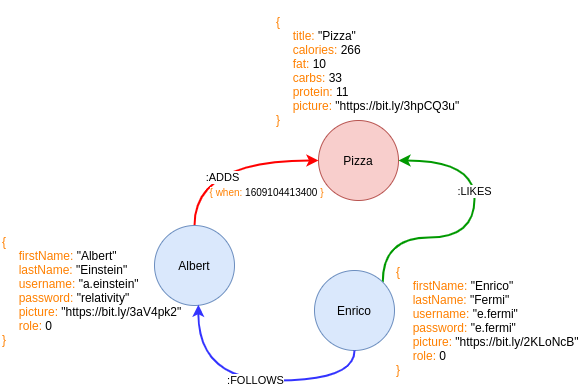
\includegraphics[scale=0.6]{img/graphDbModel.png}
	\caption{Example of GraphDB nodes and relationships}
\end{figure}

\noindent The GraphDB relationships are:
\begin{itemize}
	\item \textbf{Adds}: if the user \emph{A} has added the recipe \emph{R}, then we have a relationship \emph{:ADDS} from \emph{A} to \emph{R} ($A \rightarrow R$).
	
	\noindent We have as property, the one called \emph{when} that is the timestamp which indicates when the recipe has been added.
	
	\item \textbf{Follows}: if the user \emph{A} has followed the user \emph{B}, then we have a relationship \emph{:FOLLOWS} from \emph{A} to \emph{B} ($A \rightarrow B$).
	
	\item \textbf{Likes}: if the user \emph{A} has liked the recipe \emph{R}, then we have a relationship \emph{:LIKES} from \emph{A} to \emph{R} ($A \rightarrow R$).
\end{itemize}  

\noindent All the relationships that starts from a node \emph{X} are deleted if \emph{X} has deleted, furthermore if \emph{X} is a user, also the recipes that he has added will be eliminated. In figure 2.4 we can see an example of the nodes, the relationships and the attributes.


\subsection{Data Among Databases}
Because of the large amount of information to deal with, it is important to split up them in a way that allow us to handle them in the faster and easiest way, in order to have a good \emph{usability}. Summing up the concepts exploited so far we have the following storing strategy:
\begin{itemize}
	\item User: stored only on GraphDB
	\item Recipe: stored on DocumentDB and partially on GraphDB
\end{itemize}

\noindent The reason why we store recipes on both databases is because we want to retrieve social network information from it (likes, suggested recipes based on who added it, and so on). Hence we store on Graph DB a part of the recipe information, and the whole information about recipes on DocumentDB. This partial view of the recipe is the so-called \emph{recipe snapshot}. Also for the user exist a snapshot but it exists for implementation reason, in fact in this case all the information about the user are on GraphDB but only a part is in the snapshot. Generally speaking a snapshot is a partial view of an entity (User or Recipe). When the user clicks on the snapshot then he will see all the information (so for what concerns the recipes, the snapshot is done with GraphDB and the detailed page with DocumentDB).

\noindent We can see the storing strategy also in figure 2.5.

\begin{figure}[htpb]
	\centering
	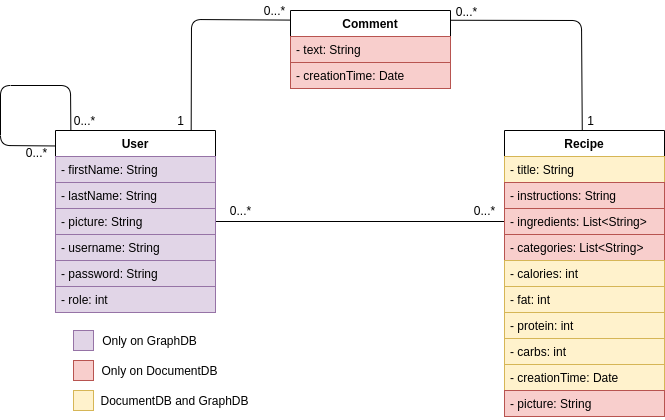
\includegraphics[scale=0.5]{img/UML_colorato.png}
	\caption{Storing Strategy}
\end{figure}

\noindent Another important detail on the Data Model is that we have chosen MongoDB as DBMS for the DocumentDB and Neo4j as DBMS for the GraphDB.

\section{Distributed Database Design}
In our application some of the most important requirements are the \emph{Availability} and the \emph{Consistency}. Thus is very important to us to have a distributed system in order to ensure:
\begin{itemize}
	\item An high availability, due to the fact that we have more servers (in our case we have 3 virtual machines provided by University of Pisa\footnote{172.16.3.157 - 172.16.3.107 -  172.16.3.108}) and so we haven't the single point of failure issue.
	\item An high consistency, because, even if the data on a server would be corrupted (for a server malfunction for instance), we have an update replica that maintains the correct data (see also 2.5.2).
	\item A low latency, in fact thanks to sharding and replicas the load is balanced among the cluster servers. We have to remark that this is not always true because, in order to maintain consistency, it is possible to have a longer latency with respect to the one that we would achieve without consistency (replicas must be updated and this requires time).
\end{itemize}

\noindent This two objectives can be reached using replicas (copy of the same data on different servers) and sharding (the dataset is split up into different parts, each part is on a different server of the cluster or on more than one server depending from the design choises performed).

\noindent In the following sections we discuss about these two techniques explaining the design choices performed in order to obtain the best performance achievable and in order to respect the given requirements. 

\subsection{Replicas}
We decide to use replicas of the same data in order to ensure \emph{availability} and \emph{consistency}. Nevertheless we have to point out that replicas alone don't ensure consistency, because it's possible to have one or more replicas that are not updated, this doesn't happen in our case because \emph{in order to commit a write operation all replicas must be updated}. This because the application is mainly read-heavy and so we need fast reads operation and, in order to achieve this, we can accept slow write operations. Moreover, this configuration ensures the \emph{Consistency} requirement.

\noindent \noindent In particular 3 replicas are present in our system: one for each machine of the provided cluster. However in our implementation only for MongoDB we have three replicas, for Neo4J we have only one instance running on server 172.16.3.107: theoretically speaking the Neo4J replicas must be three but it's a premium feature.

\noindent So, in order to sum up, let's point out in the following list, the most important points about replicas that must be taken into account.
\begin{itemize}
	\item 3 replicas for MongoDB, one for each server of the cluster
	\item 1 instance for Neo4J on 172.16.3.107
	\item All replicas must be updated in order to commit a write operation
\end{itemize}

\noindent The commands that were used to set the cluster configuration for MongoDB on the virtual machines will now be shown. It was decided to give the lowest priority to the machine running Neo4j (172.16.3.107), for load balancing. The highest priority machine is 172.16.3.157, followed by 172.16.3.108.
\begin{lstlisting}
	rsconf = 
	{
		_id: "lsmdb", 
		members: 
		[
			{
				_id: 0, 
				host: "172.16.3.157:27020", 
				priority: 2
			}, 
			{
				_id:1, 
				host: "172.16.3.107:27020", 
				priority: 0.5
			}, 
			{
				_id:2, 
				host:"172.16.3.108:27020", 
				priority: 1
			}
		], 
		settings: 
		{
			getLastErrorDefaults: 
			{
				w: 3, 
				wtimeout: 5000
			}
		}
	};	
\end{lstlisting} 

\noindent As it was expressly requested in the project documentation, a local cluster was also implemented, thanks to which it was possible to test the use of the application even with replicas on Neo4j, in addition of course to those for MongoDB.

\subsection{Sharding}
It's possible to use the following fields as shard key (because they are present in all documents of the collection):
\begin{itemize}
	\item Object ID (provided by MongoDB)
	\item Title
	\item Creation Time
	\item Instructions
	\item Ingredients
\end{itemize}

\noindent Using \emph{Instructions} and \emph{Ingredients} has no sense. For what concerns the creation time we search for the most time the most recent recipes, so if we would use it as shard key, we will access always to the shard that contains the last added recipes and the sharding strategy will be unbalanced and so it is useless. At the end we choose the \emph{Object ID} provided by Mongo because it is an automatically generated value which is better than the \emph{Title} that is inserted by the user.


\section{Software Architecture}
In this section the aspects related to the software architecture will be considered, mainly by analyzing the division of tasks between the various modules of the application. The main language used in developing the application is Java.
\subsection{Client - Server Architecture}
The application was implemented as a client-server architecture, with middleware implemented on the client side.
\subsubsection{Client Side}
The client features can be divided into two modules:
\begin{itemize}
\item The front-end module, which consists of a graphical interface based on JavaFX, which allows the users to use the application in the simplest way possible. This is critical to the usability requirement.
\item A middleware module, needed to interface the client with the server. More precisely, a driver has been implemented to interface with MongoDB and one to interface with Neo4j.
\end{itemize}
\noindent The application was developed following the MVC (Model, View, Controller) pattern. The View displays the data contained in the model and was mainly developed using .fxml files, which allow you to write all the graphic components and their properties in separate files. The Model provides methods for accessing data useful for the application. The Controller receives the commands from the user and implements them by changing the status of the other two components. This division allowed us to completely separate the three components, for a more readable and maintainable code.

\noindent Maven was used to support the implementation of the application.

\subsubsection{Server side}
The server side, as already mentioned, consists of three virtual machines, on which MongoDB and Neo4J are executed.


\subsection{Inter-Databases Consistency}
Considering how the data was distributed between the two databases, we must consider the problem of consistency on the information that forms the snapshots of the recipes, which are the only information shared by the two databases.
The general idea is that if I have to update the data of both databases I have to consider the case where the first update is successful and the second is not (I have to undo the first operation), and the case where the first update is not successful (and therefore I don't even have to do the second).
The cases that can lead to these inconsistencies are the following:
\begin{itemize}
	\item Deleting a recipe
	\item Adding a recipe
	\item Update a recipe
	\item Deleting a user (in this case his recipes must also be deleted)
\end{itemize}

\chapter{Implementation and Test}
\section{Main Modules}
The implementation code is divided into two main modules: RecipeReader and JustRecipe.
 \begin{itemize}
	\item \emph{RecipeReader}:  is a program we wrote to get our initial dataset, extracting the information that interests us from the two initial datasets (see chapter 1). To make sense of all the recipes that were initially preloaded, 20 users were entered and the recipes were randomly divided among them.
	\item \emph{JustRecipe}:  is the actual application, whose implementation will be analyzed in more details in the next sections. 
\end{itemize}
\section{Main Packages and Classes}
In this section will be presented the main packages of JustRecipe module and the respective classes.
\subsection {it.unipi.dii.inginf.lsdb.justrecipe.config}
This package is used to handle the configuration parameters, stored in \emph{config.xml}. The schema for the validation is in the file \emph{config.xsd}. The validation is very important to be sure of the correctness of the file \emph{config.xml}.

\noindent Classes:
 \begin{itemize}
	\item \emph{ConfigurationParameters}: this class stores all the configuration parameters needed by the application. For example the IP for the Neo4j database. These values do not need to be changed, so only get methods are provided. 
\end{itemize}
\subsection {it.unipi.dii.inginf.lsdb.justrecipe.main}
This package contains the Main class, that starts the application.

\noindent Classes:
 \begin{itemize}
	\item \emph{Main}: this class extends \emph{Application} and implements the \emph{start} method. 
\end{itemize}
\subsection{it.unipi.dii.inginf.lsdb.justrecipe.model}
This package contains the classes required for the model. These classes are the java bean for our application.

\noindent Classes:
  \begin{itemize}
	\item \emph{Comment}: This class stores all the information about a comment, like the text, the username of the author and the timestamp of creation. 
	\item \emph{Recipe}: This class stores all the information about a recipe, like the title, the ingredients, and so on.
	\item \emph{User}: This class stores all the information about a user, like the username, the password, and so on.
	\item \emph{Session}: This class is used to maintain the information of the session, like the logged user. We used the singleton design pattern for this class.
\end{itemize}
\subsection {it.unipi.dii.inginf.lsdb.justrecipe.persistence}
This package deals with managing the persistence of data, in fact it contains the classes used to interface with databases.

\noindent Classes:
 \begin{itemize}
	\item \emph{DatabaseDriver}: this \emph{interface} declares all the methods that has to be implemented in a database driver. This methods are \emph{initConnection()} and \emph{closeConnection()}.  
	\item \emph{MongoDBDriver}: this class implements DatabaseDriver and is responsible for implementing all the queries that have to be run on MongoDB. We used the Singleton design pattern, because a single instance of this driver must be shared by all application classes. 
	\item \emph{Neo4jDriver}: this class implements DatabaseDriver and is responsible for implementing all the queries that have to be run on Neo4j. We used the Singleton design pattern, because a single instance of this driver must be shared by all application classes.
\end{itemize}
\subsection {it.unipi.dii.inginf.lsdb.justrecipe.controller}
This package contains the classes required for the controller part of the MVC pattern. For each different page to be shown to the user, a special controller has been implemented, which manages the events resulting from the actions taken by the user and updates the model and the view.

\noindent Classes:
 \begin{itemize}
	\item \emph{WelcomePageController}: this class manages the login/register page of the application.
	\item \emph{HomePageController}: this class handles the homepage section of the application (shows the recipes of following users and handles the event, like the click on a recipe snapshot).
	\item \emph{DiscoveryPageController}: this class manages the discovery section of the application. So it is in charge of showing the results of search made by the user.
	\item \emph{ProfilePageController}: this class manages the profile section of the application. The profile could be either mine or someone else's. Thanks to this class it is possible to manage some events such as following a user, deleting my profile, seeing his recipes, and so on.
	\item \emph{AdministrationPageController}: this class handles the Administration section of the application. Of course, not all the users can access to this page, only the moderator (for seeing the last comments) and the administrators (for doing all the possible operations) can access.
	\item \emph{EditProfilePageController}: this class manages the page for editing the personal profile. The user can insert a new profile image, change the personal information, and so on. The administrator can change the role of the user in this page.
	\item \emph{AddRecipePageController}: this class manages the page of the application used for insert a new recipe. 
	\item \emph{RecipeSnapshotController}: this class manages the single recipe snapshot, like the click on him.
	\item \emph{RecipePageController}: this class handles the page in which we show all the information about a recipe. In this page it is possible also to comment a recipe and see the comments already done.
	\item \emph{CommentController}: this class manages the single comment and all the operations that can be done on him.
	\item \emph{UserSnapshotController}: this class manages the single snapshot of one user, and all the operations that can be done on him.
\end{itemize}
\subsection {it.unipi.dii.inginf.lsdb.justrecipe.utils}
This package contains a class used to store all the utility functions that we use in the application.

\noindent Classes:
 \begin{itemize}
	\item \emph{Utils}: this class is used for containing some utility functions used inside the application (to avoid code replication).
\end{itemize}

\section{Constraints}
Constraints have been added in the two databases, for the recipe title and for the user's username, which must be unique and always present.
\begin{itemize}
	\item Constraint on the \emph{title} of the recipe (on MongoDB): 
	\lstset{ language=java}
	\begin{lstlisting}
	db.recipes.createIndex (
		{
			title:1
		},
		{
			unique: true,
			name: "title_constraint"
		}
	)	
	\end{lstlisting} 
	\item Constraint on the \emph{title} of the recipe (on Neo4j): 
	\begin{lstlisting}
	CREATE CONSTRAINT title_constraint 
	ON (r:Recipe) 
	ASSERT ( r.title) IS NODE KEY	
	\end{lstlisting} 
	\item Constraint on the \emph{username} of the user: 
	\lstset{ language=java}
	\begin{lstlisting}
	CREATE CONSTRAINT username_constraint 
	ON (u:User) 
	ASSERT (u.username) IS NODE KEY	
	\end{lstlisting} 
\end{itemize}
\section{Most Relevant Queries}
In the following section will be presented the most relevant query performed with MongoDB and Neo4J. 
\noindent Some important point must be underlined:
\begin{itemize}
	\item The operation of \emph{skip} and \emph{limit}, use in the most of the following queries, are necessary due  to implementation reasons. In fact the results are not shown all in the same page (because of the size of the database the output can be huge) but only a subset of the result are shown (for instance, the first X) and in order to go on and see the other result, the query will be performed with different value of \emph{<howManyToSkip>} (the first time is 0, the second is X, the third 2X and so on) and \emph{<howManyToGet>} (it's a fixed number, must be equal to the previous X)
	\item In Neo4J part, due to performance reasons, some queries compute also followers, followings and recipes added by each user. This is necessary because when the user is given as result this information must be showed and if we don't compute it here we have to do another query for each user.
\end{itemize}

\subsection{MongoDB}

\subsubsection{Search Recipes given a username}

This query gives the opportunity to collect all the recipes written by a specific User through checking the author username field. This search is case sensitive cause we are using the username.
\begin{itemize}
	\item Input: a string who represent an username (unique through the users), how many recipe to skip, and how many to get.
	\item Output: a list of recipes, all added by the user erlier selected, ordered by the .
\end{itemize}
\lstset{ language=C++}
\begin{lstlisting}
db.recipes.aggregate (
	[
		{ 
			$match : 
			{ 
				authorUsername: <authorUsername>
			}  
		},
		{ 
				$sort : 
			{ 
				creationTime : -1 
			} 
		},
		{ 
			$skip: <howManyToSkip> 
		},
		{ 
			$limit: <howManyToGet> 
		}	
		]
)
\end{lstlisting}
\subsubsection{Search for recipe title}
Given a portion of the title, this query is capable of returning as a result a set of recipes whose titles contain it. Research must be case insensitive (see \emph{options:"i"} in the match step of the aggregation)
\begin{itemize}
\item Input: portion of the title, how many recipes to skip and how many recipes to get.
\item Output: set of recipes.	
\end{itemize}
\lstset{ language=java}
\begin{lstlisting}
db.recipes.aggregate (
	[
		{ 
			$match : 
			{ 
				title: 
				{
					$regex: /^.*<portionOfTheTitle>.*$/,
					$options: "i"
				} 
			}  
		},
		{ 
			$sort : 
			{ 
				creationTime : -1 
			} 
		},
		{ 
			$skip: <howManyToSkip> 
		},
		{ 
			$limit: <howManyToGet> 
		}	
	]
)
\end{lstlisting} 

\subsubsection{Get the username of the most versatile user}
This query let select the most versatile user, the one who had covered more recipe categories (if he/she added at least 5 different recipe in a \emph{category}, than this \emph{category} is covered).

\noindent The users are sorted by the number of distinct categories. If users have the same number of distinct categories the lexicographic order is taken into account.

\begin{itemize}
	\item Input: \emph{no input} 
	\item Output: For this early implementation of this application, we need only the best most versatile user (the first one, his/her username)
\end{itemize}
\begin{lstlisting}
db.recipes.aggregate
(
	[
		{ 
			$unwind : "$categories" 
		},
		{
			$group :
			{
				_id:
				{
					"author":"$authorUsername",
					"category":"$categories"
				},
				numRecipe:
				{
					$sum:1
				}
			}
		},
		{
			$match: 
			{
				numRecipe:
				{
					$gte: 5
				}
			}
		},
		{
			$group :
			{
				_id : "$_id.author",
				distinctCategories: 
				{ 
					$sum: 1
				}
			}
		},
		{
			$project: 
			{
				'username': '$_id',
				distinctCategories: 1,
				_id: 0
			}
		},
		{ 
			$sort : 
			{
				distinctCategories: -1,
				username: 1 
		
			} 
		},
		{ 
			$limit: 1
		}	
	]
)
\end{lstlisting}

\subsubsection{Search for recipe category}
Given the category, or a part of this, the query returns recipes that belong to it. The search is case insensitive.

\noindent It's important to point out that a recipe belongs to more than one categories, so a recipe can be part of the result of the search of two different categories (this is normal and it is allowed). 

\begin{itemize}
	\item Input: portion of the category or the entire one \emph{<portionOfTheCategory>}, how many recipes to skip \emph{<howManyToSkip>} and how many to get \emph{<howManyToGet>}.
	\item Output: set of recipes belonging to the given category
\end{itemize}
\begin{lstlisting}
db.recipes.aggregate (
	[
		{ 
			$match : 
			{ 
				categories: 
				{
					$regex: /^.*<portionOfTheCategory>.*$/,
					$options: "i"
				} 
			}  
		},
	{ 
		$sort : 
		{ 
			creationTime : -1 
		} 
	},
	{ 
		$skip: <howManyToSkip> 
	},
	{ 
		$limit: <howManyToGet> 
	}	
	]
)
\end{lstlisting}

\subsubsection{Search for recipe ingredients}
This query give the possibility to find a specific number of recipes given some of the recipe ingredients (or a portion of them). The search is case insensitive for a more easy to use experience.
\begin{itemize}
	\item Input: a list of ingredients, how many recipes to skip and how many recipe to show.
	\item Output: a list of recipes, all of them have at least all the ingredients specified before. The results are ordered from the newer to the older recipe.
\end{itemize}
It is important to say that there will be a \emph{match} step for each ingredients specified by the user.
\lstset{ language=java}
\begin{lstlisting}
	db.recipes.aggregate (
	[
	{ 
		$match : 
		{ 
			ingredients: 
			{
				$regex: /^.*<ingredients[i]>.*$/,
				$options: "i"
			} 
		}  
	},
	{ 
		$sort : 
		{ 
			creationTime : -1 
		} 
	},
	{ 
		$skip: <howManyToSkip> 
	},
	{ 
		$limit: <howManyToGet> 
	}	
	]
 )
\end{lstlisting} 

\subsubsection{Most common recipe categories}
This query allows you to get a ranking of the categories most used by users for their recipes.
\begin{itemize}
\item Input: how many categories to skip, how many categories to get.
\item Output: list with the categories ordered by the number of use.
\end{itemize}
\lstset{ language=java}
\begin{lstlisting}
db.recipes.aggregate (
	[
		{ 
			$unwind : "$categories" 
		},
		{
			$group :
			{
				_id : "$categories",
			 	numberOfRecipes: 
				{ 
					$sum: 1
				 }
			}
		},
		{
			$project: 
			{
				'category': '$_id',
				numberOfRecipes: 1,
				_id: 0
			}
		},
		{ 
			$sort : 
			{ 
				numberOfRecipes : -1 
			} 
		},
		{ 
			$skip: <howManyToSkip> 
		},
		{ 
			$limit: <howManyToGet> 
		}	
	]
)
\end{lstlisting}

\subsubsection{Last Comments}
The query returns the last comments sorted for creation time, in order to have the most recent as first and the most old as last.

\begin{itemize}
	\item Input: \emph{howManyToGet} and \emph{howManyToSkip}
	\item Output: set of the last comments sorted by creation time in descendant order.
\end{itemize}

\begin{lstlisting}
db.recipes.aggregate (
	[
		{ 
			$unwind : "$comments" 
		},
		{ 
			$sort : 
			{ 
				"comments.creationTime" : -1 
			} 
		},
		{ 
			$skip: <howManyToSkip> 
		},
		{ 
			$limit: <howManyToGet> 
		}	
	]
)
\end{lstlisting}

\subsubsection{Weekly Recipes per User}
A query who returns all the recipes between two dates, first day of the week and first day of the next week.
\begin{itemize}
	\item Input: \emph{Username} who represent the user.
	\item Output: set of recipes which the user has added in the current week.
\end{itemize}

\begin{lstlisting}
	db.recipes.aggregate {
		$match: 
			{ 
				$and: 
					[
						{
							creationTime
							{ 
								$gte: <firstDateOfWeek>,
							 	$lt: <firstDateOfNextWeek>
							}
						},
					 	{
							authorUsername: <username>
						}
					]
			}
		}
\end{lstlisting}

\newpage
\subsection{Neo4J}
Now we will talk about the queries on Neo4j, but first we need to consider their domain-specific to graph-centric translation.
\begin{table}[htpb]
\caption{Graph-Centric Query and Domain-Specific Query}
\centering
\begin{tabular}{|l|l|}
\hline
\rowcolor[HTML]{000000} 
{\color[HTML]{FFFFFF} Graph-Centric Query} & {\color[HTML]{FFFFFF} Domain-Specific Query} \\ \hline
\begin{tabular}[c]{@{}l@{}}How many incoming edges are incident \\ to vertex A? \end{tabular}& \begin{tabular}[c]{@{}l@{}}How many users follow one user? \\ How many likes has a recipe received?\end{tabular} \\ \hline
\begin{tabular}[c]{@{}l@{}}How many hops does it take to get from \\ vertex A to vertex B?\end{tabular} & \begin{tabular}[c]{@{}l@{}}How many follows relations are between \\ User A and User B? \\(used within the search for suggested recipes)\end{tabular} \\ \hline
\begin{tabular}[c]{@{}l@{}}What is the centrality measure of vertex B? \\ (How well connected is?)\end{tabular} & \begin{tabular}[c]{@{}l@{}}Most followed and active users, Best recipes,\\ Most liked users\end{tabular} \\ \hline
\end{tabular}
\end{table}

\noindent A partial example of a graph (screenshot made during the execution of the program) is shown in the figure 3.1 , in order to have more clear the concepts that will be expressed later in the implementation of the queries.
\begin{figure}[htpb]
	\centering
	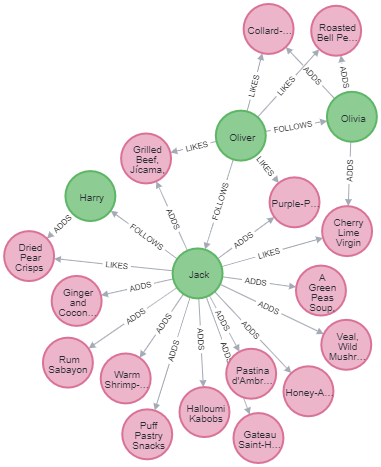
\includegraphics[scale=0.7]{img/graphScreen.png}
	\caption{Partial example of the graph in Neo4j}
\end{figure}


\subsubsection{Suggested Recipes}
We have two levels of suggestions with different relevance.
\begin{itemize}
	\item First Level
	
	\noindent Recipe \emph{R} is a first level suggestion for the user \emph{X}, if \emph{R} has been added by the user \emph{Y} where \emph{Y} is followed by \emph{W} who is followed by \emph{X} ($X \rightarrow W \rightarrow Y$). Or \emph{R} has been added by \emph{Z} where \emph{Z} is followed by \emph{Y} ($ X \rightarrow W \rightarrow Y \rightarrow Z$).
	
	\item Second Level
	
	\noindent Recipe \emph{R} is a second level suggestion for the user \emph{X} if \emph{R} has been added by the user \emph{Y} where \emph{Y} is the owner of at least N recipes liked by \emph{X}.
	
\end{itemize}


\noindent The two level of suggestions are in a single query, the first recipes are the ones related to the first level, then at the end we have the ones related to the second level. The code is show below:

\begin{lstlisting}
	MATCH path =
	(recipe:Recipe)<-[a:ADDS]-(owner:User)<-[:FOLLOWS*2..3]
	-(me:User{username:$u})
	WHERE owner.username <> $u
	RETURN recipe.title, recipe.calories, recipe.carbs,
	recipe.protein, recipe.fat, recipe.picture,
	a.when, owner.username
	ORDER BY length(path) ASC, a.when DESC
	SKIP $howManyToSkipFirstLv
	LIMIT $howManyToGetFirstLv
	UNION
	MATCH (:User{username:$u})-[l:LIKES]->(:Recipe)<-[:ADDS]-
	(owner:User)
	WITH DISTINCT(owner) AS owner, COUNT(DISTINCT l) AS numLikes
	WHERE numLikes > $threshold AND owner.username <> $u
	MATCH (owner)-[a:ADDS]->(recipe:Recipe)
	RETURN recipe.title, recipe.calories, recipe.carbs,
	recipe.protein, recipe.fat, recipe.picture, a.when,
	owner.username
	ORDER BY a.when DESC
	SKIP $howManyToSkipSecondLv
	LIMIT $howManyToGetSecondLv	
\end{lstlisting}

\subsubsection{Recipes of following users}
This query returns all the recipes of the following users of a specific user.
\begin{itemize}
	\item Input: How many recipe name to skip, how many recipe name to show and a string who represents a specific username.
	\item Output: A set of recipe name of the specific user's following users have added.
\end{itemize}
\lstset{ language=java}
\begin{lstlisting}
	MATCH (u1:User{username:$username})-[:FOLLOWS]->(u2:User)-[a:ADDS]->(r:Recipe)
	RETURN r.title AS title, r.calories AS calories,
		 r.fat AS fat, r.protein AS protein, r.carbs AS carbs,
		 r.picture AS picture, u2.username AS authorUsername 
	ORDER BY a.when DESC 
	SKIP $skip LIMIT $limit
\end{lstlisting}
\subsubsection{Most followed and active users}
This query returns the list of the most followed and active users, namely the influencers.
Most followed means that the list is ordered by the number of followers.
Active means that the list is ordered by the number of recipes added by the user.
\begin{itemize}
	\item Input: How many users to skip, how many users to show.
	\item Output: A list of the most followed and active users.
\end{itemize}
\lstset{ language=java}
\begin{lstlisting}
	MATCH (u:User)
	OPTIONAL MATCH (u)<-[f1:FOLLOWS]-(:User)
	OPTIONAL MATCH (u)-[f2:FOLLOWS]->(:User)
	OPTIONAL MATCH (u)-[a:ADDS]->(:Recipe)
	RETURN u.firstName, u.lastName, u.username, 
		u.firstName AS firstName, u.lastName AS lastName, 
		u.picture AS picture, u.username AS username,
		u.password AS password, u.role AS role,
	COUNT(DISTINCT f1) AS follower,
	COUNT(DISTINCT f2) AS following,
	COUNT(DISTINCT a) AS numRecipes
	ORDER BY follower DESC, numRecipes DESC
	SKIP $howManySkip LIMIT $howMany
\end{lstlisting}
\subsubsection{Most liked users}
This query returns the list of the most liked users, namely the users who received more like to their recipes.
\begin{itemize}
	\item Input: How many users to skip, how many users to show.
	\item Output: A list of the most liked users.
\end{itemize}
\lstset{ language=java}
\begin{lstlisting}
	MATCH (u:User)
	OPTIONAL MATCH (u)-[:ADDS]->(:Recipe)<-[l:LIKES]-(:User)
	OPTIONAL MATCH (u)<-[f1:FOLLOWS]-(:User)
	OPTIONAL MATCH (u)-[f2:FOLLOWS]->(:User) 
	OPTIONAL MATCH (u)-[a:ADDS]->(:Recipe)
	RETURN u.firstName, u.lastName, u.username, 
		u.firstName AS firstName, u.lastName AS lastName, 
		u.picture AS picture, u.username AS username, 
		u.password AS password, u.role AS role, 
	COUNT(DISTINCT f1) AS follower, 
	COUNT(DISTINCT f2) AS following, 
	COUNT(DISTINCT a) AS numRecipes, 
	COUNT(DISTINCT l) AS totLikes 
	ORDER BY totLikes DESC 
	SKIP $howManySkip LIMIT $howMany
\end{lstlisting}
\subsubsection{Best Recipes}
This query returns the list of the best recipes, namely the most liked ones.
\begin{itemize}
	\item Input: How many recipes to skip, how many recipes to show.
	\item Output: A list of the best recipes.
\end{itemize}
\lstset{ language=java}
\begin{lstlisting}
	MATCH (:User)-[l:LIKES]->(r:Recipe)
	MATCH (u:User)-[:ADDS]->(r)
	RETURN r.title AS title, r.calories AS calories,
		r.fat AS fat, r.protein AS protein, r.carbs AS carbs, 
		r.picture AS picture, u.username AS authorUsername,
	COUNT(DISTINCT l) AS likes 
	ORDER BY likes DESC
	SKIP $skip LIMIT $limit
\end{lstlisting}
To clarify, the first match is used to avoid to consider the recipes which have not at least one like, and the second match is used to find the user that adds the recipe.
\subsubsection{Search for username}
Given a portion of the username, this query is able to return all users whose usernames contain it. The search must be case insensitive, so the toLower function is used. 
\begin{itemize}
\item Input: portion of the username, how many users to skip and how many users to get.
\item Output: set of users.	
\end{itemize}
\lstset{ language=java}
\begin{lstlisting}
	MATCH (u:User)
	WHERE toLower(u.username) CONTAINS toLower($username)
	OPTIONAL MATCH (u)<-[f1:FOLLOWS]-(:User)
	OPTIONAL MATCH (u)-[f2:FOLLOWS]->(:User)
	OPTIONAL MATCH (u)-[a:ADDS]->(:Recipe)
	RETURN u.firstName AS firstName, u.lastName AS lastName, 
		u.picture AS picture, u.username AS username, 
		u.password AS password, u.role AS role, 
	COUNT(DISTINCT f1) AS follower,
	COUNT(DISTINCT f2) AS following, 
	COUNT(DISTINCT a) AS numRecipes
	SKIP $skip LIMIT $limit
\end{lstlisting} 
\subsubsection{Search for user's full-name}
Given the full-name or a part of it, the query returns the users that contains in their full-name the given input. The query is case-insensitive.
\begin{itemize}
	\item Input: The full-name (\emph{\$fullName}), how many users to skip (\emph{\$skip}) and how many users to get (\emph{\$limit}).
	\item Output: The users that contains in their full-name the given input \emph{\$fullName}.
\end{itemize}
\begin{lstlisting}
	 MATCH (u:User) 
	 WHERE
	 toLower(u.firstName+' '+u.lastName)
	 CONTAINS toLower($fullName)
	 OR
	 toLower(u.lastName + ' ' + u.firstName)
	 CONTAINS toLower($fullName)
	 OPTIONAL MATCH (u)<-[f1:FOLLOWS]-(:User)
	 OPTIONAL MATCH (u)-[f2:FOLLOWS]->(:User)
	 OPTIONAL MATCH (u)-[a:ADDS]->(:Recipe)
	 RETURN u.firstName AS firstName, u.lastName AS lastName,
	 	u.picture AS picture, u.username AS username,
	 	u.password AS password, u.role AS role,
	 COUNT (DISTINCT f1) AS follower,
	 COUNT (DISTINCT f2) AS following,
	 COUNT (DISTINCT a) AS numRecipes
	 SKIP $skip LIMIT $limit
\end{lstlisting} 

\section {Some snapshots of code}
Some interesting snapshots of the code will be showed.
\subsection{Most relevant queries}
The implementation code in Java language of the most interesting queries among those seen in the previous section will also be shown.
\subsubsection{Get the username of the most versatile user}
\lstset{language=code}
\begin{lstlisting}
public String searchMostVersatileUser(final int recipesThreshold)
{
  Bson unwind = unwind("$categories");
  Bson group = new Document("$group", 
    new Document("_id", 
      new Document("author", "$authorUsername")
        .append("category", "$categories"))
        .append("numRecipe", new Document("$sum", 1)));
  Bson match = match(gte("numRecipe", recipesThreshold));
  Bson group2 = group("$_id.author", sum("distinctCategories", 1));
  Bson project = project(fields(computed("username", "$_id"), 
    excludeId(), include("distinctCategories")));
  Bson sortNumName = new Document("$sort", new Document("distinctCategories", -1).append("username", 1));
  Bson limit = limit(1);

  Document doc = (Document) collection.aggregate(
    Arrays.asList(unwind, group, match, group2, project, 
    sortNumName, limit)).first();

  return doc.getString("username");
}	
\end{lstlisting} 
\subsubsection{Most common recipe categories}
\lstset{language=code}
\begin{lstlisting}
public List<String> searchMostCommonRecipeCategories (final int howManySkip, final int howManyCategories)
{
    List<String> mostCommonCategories = new ArrayList<>();
    Bson unwind = unwind("$categories");
    Bson group = group("$categories", Accumulators.sum("numberOfRecipes", 1));
    Bson project = project(fields(computed("category", "$_id"), 
      excludeId(), include("numberOfRecipes")));
    Bson sort = sort(descending("numberOfRecipes"));
    Bson skip = skip(howManySkip);
    Bson limit = limit(howManyCategories);
    List<Document> results = (List<Document>) collection.aggregate(
      Arrays.asList(unwind, group, project, sort, skip, limit))
        .into(new ArrayList());

    for (Document document: results)
    {
        mostCommonCategories.add(document.getString("category"));
    }
    return mostCommonCategories;
}	
\end{lstlisting} 
\subsubsection{Last comments}
\lstset{language=code}
\begin{lstlisting}
public List<List<Object>> searchAllComments (final int howManySkip,final  int howMany)
{
	List<List<Object>> objects = new ArrayList<>();
	Gson gson = new Gson();
	Bson unwind = unwind("$comments");
	Bson sort = sort(descending("comments.creationTime"));
	Bson skip = skip(howManySkip);
	Bson limit = limit(howMany);
	MongoCursor<Document> iterator = (MongoCursor<Document>)
	  collection.aggregate(Arrays.asList(unwind, sort, skip, limit)).iterator();
	while (iterator.hasNext())
	{
		Document document = iterator.next();
		Document commentDocument = (Document) document.get("comments");
		Comment comment = gson.fromJson(gson.toJson(commentDocument),Comment.class);
		// I need to re-obtain the full recipe
		Recipe recipe = getRecipeFromTitle(document.getString("title"));

		List<Object> objectList = new ArrayList<>();
		objectList.add(comment);
		objectList.add(recipe);

		objects.add(objectList);
	}
	return objects;
}
\end{lstlisting} 
\subsubsection{Suggested recipes}
\lstset{language=code}
\begin{lstlisting}
public List<Recipe> getSuggestedRecipes(final String username, final int threshold, final int howManyToSkipFirstLv, final int howManyToGetFirstLv, final int howManyToSkipSecondLv, final int howManyToGetSecondLv)
{
	List<Recipe> recipes = new ArrayList<>();
	try(Session session = driver.session()) 
	{
		recipes = session.readTransaction((TransactionWork<List<Recipe>>) tx -> 
		{
			Result result = tx.run("
			MATCH path = (recipe:Recipe)<-[a:ADDS]-
			  (owner:User)<-[:FOLLOWS*2..3]-(me:User{username:$u}) 
			WHERE owner.username <> $u 
			RETURN recipe.title, recipe.calories, recipe.carbs, recipe.protein, 
			  recipe.fat, recipe.picture, a.when, owner.username 
			ORDER BY length(path) ASC, a.when DESC 
			SKIP $firstLvSkip LIMIT $firstLvGet 
			UNION 
			MATCH (:User {username: $u})-[l:LIKES]->(:Recipe)
			  <-[:ADDS]-(owner:User) 
			WHERE owner.username <> $u 
			WITH DISTINCT(owner) AS owner, COUNT(DISTINCT l) AS numLikes 
			WHERE numLikes > $treshold AND owner.username <> $u 
			MATCH (owner)-[a:ADDS]->(recipe:Recipe) 
			RETURN recipe.title, recipe.calories, recipe.carbs, recipe.protein, 
			  recipe.fat, recipe.picture, a.when, owner.username 
			ORDER BY a.when DESC 
			SKIP $secondLvSkip LIMIT $secondLvGet",
			parameters("u",username, "firstLvSkip", howManyToSkipFirstLv, 
			  "firstLvGet", howManyToGetFirstLv, "treshold", threshold, 
			  "secondLvSkip", howManyToSkipSecondLv, 
			  "secondLvGet", howManyToGetSecondLv));

			List<Recipe> r = new ArrayList<>();

			while(result.hasNext())
			{
				Record rec = result.next();
				String title = rec.get("recipe.title").asString();
				int calories = 0;
				int protein = 0;
				int fat = 0;
				int carbs = 0;
				String picture = null;
				String authorUsername = rec.get("owner.username").asString();
				if(rec.get("recipe.calories") != NULL)
					calories = rec.get("recipe.calories").asInt();
				if(rec.get("recipe.fat") != NULL)
					fat = rec.get("recipe.fat").asInt();
				if(rec.get("recipe.protein") != NULL)
					protein = rec.get("recipe.protein").asInt();
				if(rec.get("recipe.carbs") != NULL)
					carbs = rec.get("recipe.carbs").asInt();
				if (rec.get("recipe.picture") != NULL)
					picture = rec.get("recipe.picture").asString();
				Recipe recipe = new Recipe(title, fat, calories, protein, carbs, 
				  picture);
				recipe.setAuthorUsername(authorUsername);
				r.add(recipe);
			}
			return r;
		});
	}
	return recipes;
}
\end{lstlisting} 

\subsubsection{Most followed and active users}
\lstset{language=code}
\begin{lstlisting}
public List<User> searchMostFollowedAndActiveUsers (final int howManySkip, 
	final int howMany)
{
	List<User> users = new ArrayList<>();
	try(Session session = driver.session())
	{
		users = session.readTransaction((TransactionWork<List<User>>)  tx -> 
		{
			Result result = tx.run("
				MATCH (u:User) 
				OPTIONAL MATCH (u)<-[f1:FOLLOWS]-(:User) 
				OPTIONAL MATCH (u)-[f2:FOLLOWS]->(:User) 
				OPTIONAL MATCH (u)-[a:ADDS]->(:Recipe) 
				RETURN u.firstName, u.lastName, u.username, u.firstName AS firstName, 
				  u.lastName AS lastName, u.picture AS picture, u.username AS username, 
				  u.password AS password, u.role AS role, 
				  COUNT(DISTINCT f1) AS follower, 
				  COUNT(DISTINCT f2) AS following, 
				  COUNT(DISTINCT a) AS numRecipes 
				ORDER BY follower DESC, numRecipes DESC 
				SKIP $howManySkip LIMIT $howMany",
				parameters("howManySkip", howManySkip, "howMany", howMany));
			List<User> listOfUsers = new ArrayList<>();
			while(result.hasNext())
			{
				Record r = result.next();
				String firstName = r.get("firstName").asString();
				String lastName = r.get("lastName").asString();
				String picture = null;
				if (r.get("picture") != NULL)
				{
					picture = r.get("picture").asString();
				}
				String username = r.get("username").asString();
				String password = r.get("password").asString();
				int role = r.get("role").asInt();
				User user = new User(firstName, lastName, picture, username, 
				  password, role);
				user.setFollower(r.get("follower").asInt());
				user.setFollowing(r.get("following").asInt());
				user.setNumRecipes(r.get("numRecipes").asInt());
				listOfUsers.add(user);
			}
			return listOfUsers;
		});
	}
	return users;
}
\end{lstlisting}

\section{Tests and Statistical Analysis}
\subsection{Queries Analysis}
The most queries consist in read operations and so we can say that the application is read-heavy. In the table 3.2 we can see the frequency of each query. 

\begin{table}[htpb]
	\centering
	\caption{Queries Frequency}
	\begin{tabular}{|c|c|lll}
		\cline{1-2}
		\cellcolor[HTML]{000000}{\color[HTML]{FFFFFF} Query} &
		\cellcolor[HTML]{000000}{\color[HTML]{FFFFFF} Frequency} &
		\multicolumn{1}{c}{\cellcolor[HTML]{FFFFFF}{\color[HTML]{FFFFFF} }} &
		&
		\\ \cline{1-2}
		Search Recipes given a username             & High   & \cellcolor[HTML]{FFFFFF} &  &  \\ \cline{1-2}
		Search for Recipe Title                     & Medium & \cellcolor[HTML]{FFFFFF} &  &  \\ \cline{1-2}
		Get the username of the most versatile user & Low    &                          &  &  \\ \cline{1-2}
		Search for Recipe Category                  & Low    &                          &  &  \\ \cline{1-2}
		Search for Recipe Ingredients               & Low    &                          &  &  \\ \cline{1-2}
		Most Common Recipe Categories               & Low    &                          &  &  \\ \cline{1-2}
		Last Comments                               & Medium &                          &  &  \\ \cline{1-2}
		Weekly Recipes per User                     & High   &                          &  &  \\ \cline{1-2}
		Suggested Recipes                           & High   &                          &  &  \\ \cline{1-2}
		Recipes of Following Users                  & High   &                          &  &  \\ \cline{1-2}
		Most Followed an Active Users               & Low    &                          &  &  \\ \cline{1-2}
		Most Liked Users                            & Low    &                          &  &  \\ \cline{1-2}
		Best Recipes                                & Low    &                          &  &  \\ \cline{1-2}
		Search for Username                         & Medium &                          &  &  \\ \cline{1-2}
		Search for User's Full Name                 & Low    &                          &  &  \\ \cline{1-2}
	\end{tabular}
\end{table}

\subsection{Index Analysis}

In this subsection the indices for both MongoDB and Neo4J will be considered, and statistical tests will be performed to understand their benefit. For each index will be considered the queries that are in some way affected by its presence. For performance measures of Neo4j queries, the keyword \emph{PROFILE} was used at the beginning of the query, which allows you to see the steps behind the execution of the query. We have to underline that in using \emph{PROFILE} we have to neglect the first value of execution time, because this is affected by the time that Neo4J spends in executing the statistical information and he graphical output given by the command, from the second execution the time execution is reliable (the most of the previous information are already computed). For MongoDB, we used the \emph{explain()}.

\noindent The following index will be analyzed:
\begin{itemize}
	\item Recipe Title (MongoDB and Neo4j)
	\item User Username (Neo4J)
	\item Recipe Creation Time (MongoDB)
	\item Comment Creation Time (MongoDB)
\end{itemize}

\subsubsection {Index on Recipe Title}
Since a constraint on the recipe title was needed, and this was implemented with an index on it, then the index on the recipe title was not taken into account in these tests, because it is mandatory.

\subsubsection {Index on User Username}
The constraint on the username is also inserted through an index, so the index on the username is also mandatory.

\subsubsection{Index on Recipe Creation Time}
A study of performance has been completed, the results are available in table 3.2. The table displays that the index on the creation time field is a good index, which improve the performance of the application, by reducing the number of document and keys examined and reducing the execution time, for all the query considered. All the following (the ones in table 3.2) query has been tried as they could appear during the natural execution of the application. All of this query are sorted by the creation time (descending) but the first one, this consider the recipes added by a user in a date interval. This results are so good that the index tested has been implemented on MongoDB.

\begin{table}[htpb]
	\caption{Test on creationTime Index}
	\centering
	\begin{tabular}{|c|c|c|l}
		\cline{1-3}
		\cellcolor[HTML]{000000}{\color[HTML]{FFFFFF} Query} & \cellcolor[HTML]{000000}{\color[HTML]{FFFFFF} Results without Index}                                                     & \cellcolor[HTML]{000000}{\color[HTML]{FFFFFF} Results with Index}                                                        &  \\ \cline{1-3}
		Weekly Recipes per User                              & \begin{tabular}[c]{@{}c@{}}executionTimeMillis : 30,\\ totalKeysExamined : 0,\\ totalDocsExamined : 45348\end{tabular}   & \begin{tabular}[c]{@{}c@{}}executionTimeMillis : 2,\\ totalKeysExamined : 0,\\ totalDocsExamined : 0\end{tabular}        &  \\ \cline{1-3}
		Search Recipes given a username                                       & \begin{tabular}[c]{@{}c@{}}executionTimeMillis : 37,\\ totalKeysExamined : 0,\\ totalDocsExamined : 45348\end{tabular}   & \begin{tabular}[c]{@{}c@{}}executionTimeMillis : 7,\\ totalKeysExamined : 1280,\\ totalDocsExamined : 1280\end{tabular}  &  \\ \cline{1-3}
		Search for Recipe Title                              & \begin{tabular}[c]{@{}c@{}}executionTimeMillis : 57,\\ totalKeysExamined : 45348,\\ totalDocsExamined : 389\end{tabular} & \begin{tabular}[c]{@{}c@{}}executionTimeMillis : 29,\\ totalKeysExamined : 6126,\\ totalDocsExamined : 6126\end{tabular} &  \\ \cline{1-3}
		Search for recipe category                           & \begin{tabular}[c]{@{}c@{}}executionTimeMillis : 75,\\ totalKeysExamined : 0,\\ totalDocsExamined : 45348\end{tabular}   & \begin{tabular}[c]{@{}c@{}}executionTimeMillis : 2,\\ totalKeysExamined : 129,\\ totalDocsExamined : 129\end{tabular}    &  \\ \cline{1-3}
		Search for recipe ingredients                        & \begin{tabular}[c]{@{}c@{}}executionTimeMillis : 226,\\ totalKeysExamined : 0,\\ totalDocsExamined : 45348\end{tabular}  & \begin{tabular}[c]{@{}c@{}}executionTimeMillis : 32,\\ totalKeysExamined : 4591,\\ totalDocsExamined : 4591\end{tabular} &  \\ \cline{1-3}
	\end{tabular}
\end{table}


\subsubsection{Index on Comment Creation Time}
A possible index is the one on the creation time of the comment, this index affect the query \emph{Last Comments}. In order to see if the index must be added or not, let analyze the result of the index analysis for this index on that query (see table 3.3)

\begin{table}[htpb]
	\centering
	\caption{Statistics about comment creation time index}
		\begin{tabular}{lllll}
			\cline{1-3}
			\multicolumn{1}{|c|}{\cellcolor[HTML]{000000}{\color[HTML]{FFFFFF} Query}} &
			\multicolumn{1}{c|}{\cellcolor[HTML]{000000}{\color[HTML]{FFFFFF} Results without index}} &
			\multicolumn{1}{c|}{\cellcolor[HTML]{000000}{\color[HTML]{FFFFFF} Results with index}} &
			&
			\\ \cline{1-3}
			\multicolumn{1}{|l|}{Suggested Recipes} &
			\multicolumn{1}{l|}{\begin{tabular}[c]{@{}l@{}}Examined: 125843\\ Execution Time: 179ms\end{tabular}} &
			\multicolumn{1}{l|}{\begin{tabular}[c]{@{}l@{}}Examined: 125843\\ Execution Time: 113ms\end{tabular}} &
			&
			\\ \cline{1-3}
			\multicolumn{1}{|l|}{Recipes of Following Users} &
			\multicolumn{1}{l|}{\begin{tabular}[c]{@{}l@{}}Examined: 82836\\ Execution Time: 39ms\end{tabular}} &
			\multicolumn{1}{l|}{\begin{tabular}[c]{@{}l@{}}Examined: 82836\\ Execution Time: 38ms\end{tabular}} &
			&
			\\ \cline{1-3} 
		\end{tabular}
	\end{table}
\noindent From the result obtained we can see that the addition of that index do not imply a improve in the performance but instead a downgrade of performance. In fact the query with the index require more time with respect to the one without index.

\noindent For this reason we don't create an index on the creation time of the comment.

\noindent The reason for the downgrade of the performance is because MongoDB creates a multi index, so it create an index for recipe and another index for comments. Thus if the index is present it examines a number of keys that is larger than the number of recipes, because it takes into account recipes and comments.
\begin{comment}
\subsubsection{Index on Recipe Addition Time}
A possible index is the one on the attribute \emph{when} of the relations \emph{ADDS} in Neo4J database. In order to evaluate the performance of this index let analyze the test results in table 3.5 obtained using the command \emph{PROFILE} and doing repetead tests taking the mean value at the end.

\begin{table}[htpb]
	\centering
	\caption{Statistics about index on recipe addition time}
	\begin{tabular}{lllll}
		\cline{1-3}
		\multicolumn{1}{|c|}{\cellcolor[HTML]{000000}{\color[HTML]{FFFFFF} Query}} &
		\multicolumn{1}{c|}{\cellcolor[HTML]{000000}{\color[HTML]{FFFFFF} Results without index}} &
		\multicolumn{1}{c|}{\cellcolor[HTML]{000000}{\color[HTML]{FFFFFF} Results with index}} &
		&
		\\ \cline{1-3}
		\multicolumn{1}{|l|}{Suggested Recipes} &
		\multicolumn{1}{l|}{\begin{tabular}[c]{@{}l@{}}Examined: 89988\\ Mean Execution Time: 149,6ms\end{tabular}} &
		\multicolumn{1}{l|}{\begin{tabular}[c]{@{}l@{}}Examined: 89988\\ Mean Execution Time: 122ms\end{tabular}} &
		&
		\\ \cline{1-3}
		\multicolumn{1}{|l|}{Recipes of Following Users} &
		\multicolumn{1}{l|}{\begin{tabular}[c]{@{}l@{}}Examined: 13935\\ Mean Execution Time: 11ms\end{tabular}} &
		\multicolumn{1}{l|}{\begin{tabular}[c]{@{}l@{}}Examined: 13935\\ Mean Execution Time: 9,8ms\end{tabular}} &
		&
		\\ \cline{1-3}
	\end{tabular}
\end{table}

\noindent As we can see from the table only for the first query we have a little margin of benefit (for the first case we can say that the performance are equal), but this margin is not good enough (it's only 30 ms more or less) to justify the addition of this index, because even if it improves a bit the performance on the \emph{Suggested Recipes} query, it deteriorates the writing performance because we have to update the index for each insertion.
\end{comment}

\chapter{User Manual}
In this chapter we discuss how to use the application from the user's point of view.
\section{How To Configure The System}
In order to configure the application an XML file is provided, this file contains configuration parameters that can affect the proper work of the application so only in particular cases must be changed. In any case the XML file will be validated and the application doesn't work if this validation fails. The file contains the following code.

\lstset{language=code}
\begin{lstlisting}
	<?xml version="1.0" encoding="UTF-8"?>
	<it.unipi.dii.inginf.lsdb.justrecipe.config.ConfigurationParameters>
		<mongoFirstIp>172.16.3.157</mongoFirstIp>
		<mongoFirstPort>27020</mongoFirstPort>
		<mongoSecondIp>172.16.3.107</mongoSecondIp>
		<mongoSecondPort>27020</mongoSecondPort>
		<mongoThirdIp>172.16.3.108</mongoThirdIp>
		<mongoThirdPort>27020</mongoThirdPort>
		<mongoUsername></mongoUsername>
		<mongoPassword></mongoPassword>
		<mongoDbName>justrecipe</mongoDbName>
		<neo4jIp>172.16.3.107</neo4jIp>
		<neo4jPort>7687</neo4jPort>
		<neo4jUsername>neo4j</neo4jUsername>
		<neo4jPassword>justrecipe</neo4jPassword>
	</it.unipi.dii.inginf.lsdb.justrecipe.config.ConfigurationParameters>
\end{lstlisting}

\section{How To Launch The Application}
\newpage
\section{Login And Registration}
At the first launch of the application the window in figure 4.1 is shown:
\begin{figure}[htpb]
	\centering
	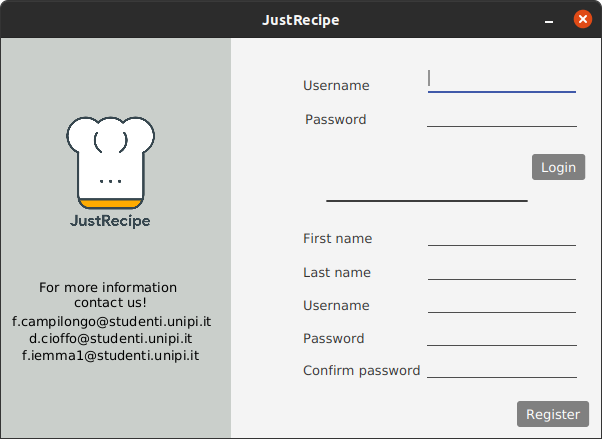
\includegraphics[scale=0.3]{img/user_manual/login.png}
	\caption{First window of the application}
\end{figure}

\noindent Now the user has two possibilities:
\begin{itemize}
	\item \textbf{if} he is already registered he can do the login
	\item \textbf{if} he is not registered yet, then he must sign-up to use the application.
\end{itemize}

\noindent Let suppose that we are in the second case. So we have to compile the registering section as is shown in the figure 4.2. Where we register the user \emph{Albert Einstein} with username \emph{a.einstein} and password \emph{a.einstein}. 

\begin{figure}[htpb]
	\centering
	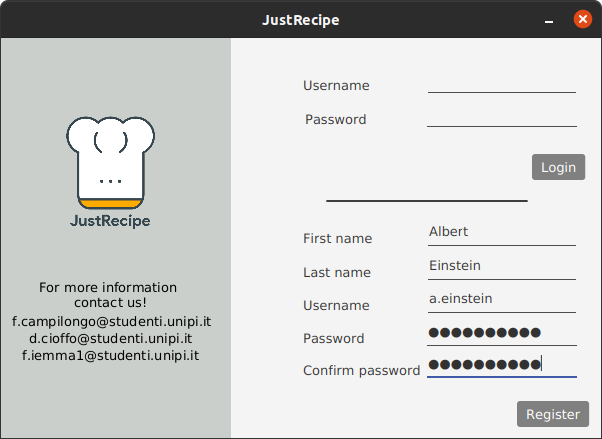
\includegraphics[scale=0.3]{img/user_manual/register.png}
	\caption{Registering section}
\end{figure}

\noindent If the user click on \textbf{Register} the user will be registered and the login is performed automatically.

\noindent If the user is already registered then he can directly sign-in using the login section as in figure 4.3.

\begin{figure}[htpb]
	\centering
	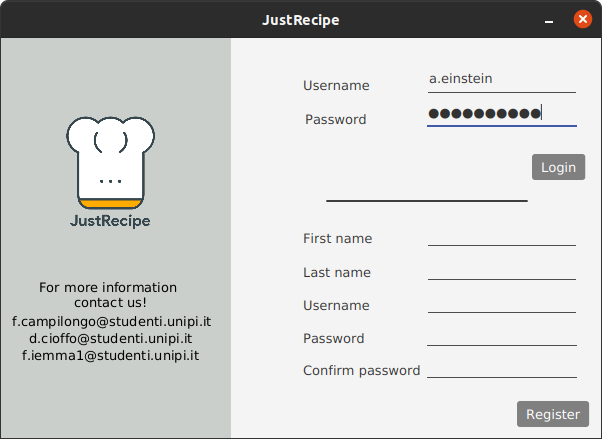
\includegraphics[scale=0.3]{img/user_manual/loginsection.png}
	\caption{Login section}
\end{figure}

\newpage
\section{Homepage, Discovery and First Steps}
Let continue with the user \emph{a.einstein}. After the login the homepage will be shown. In the homepage there are the recipes of the following users, due to the fact that the logged user is a new user, he doesn't follow anyone and so he see nothing (see figure 4.4).

\begin{figure}[htpb]
	\centering
	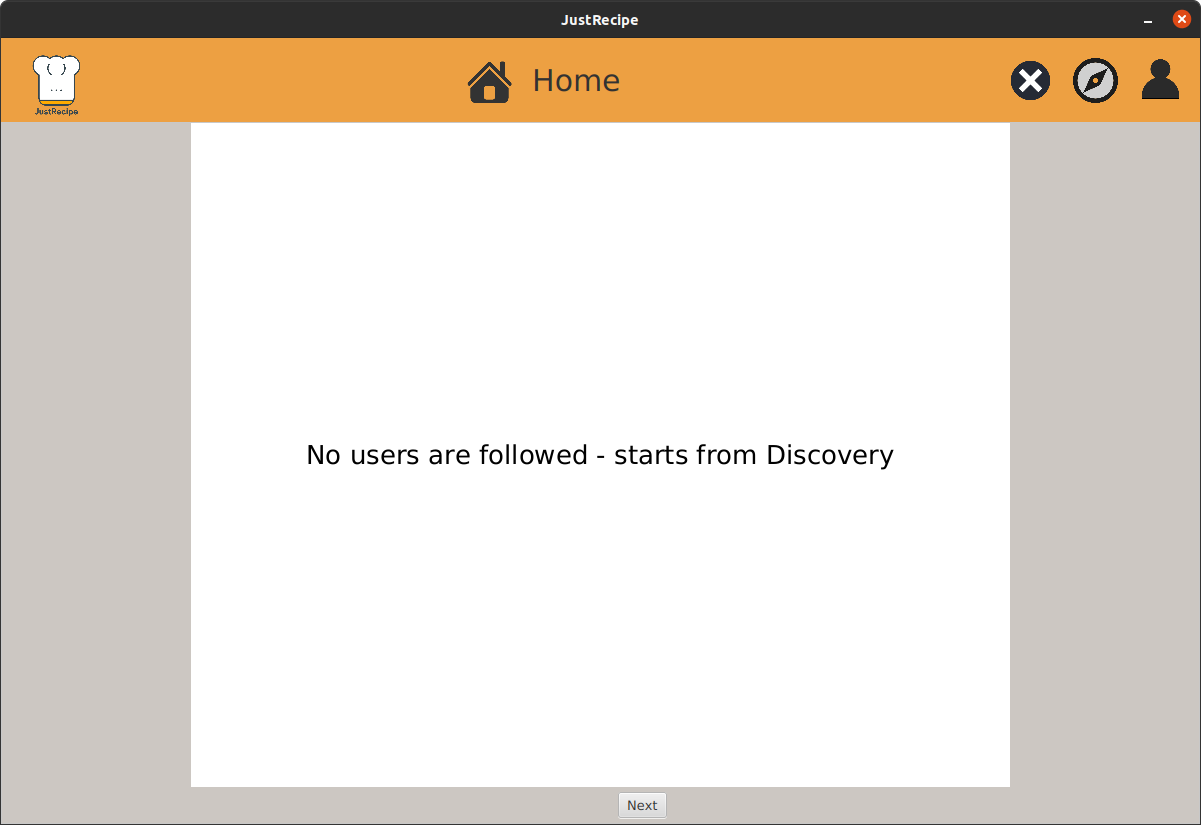
\includegraphics[scale=0.25]{img/user_manual/blank-homepage.png}
	\caption{Initial page}
\end{figure}

\noindent In order to follow other users and starts to read recipes, the user must click on the icon that represents the \textbf{Discovery} page, as shown in figure 4.5.

\begin{figure}[htpb]
	\centering
	
\includegraphics[scale=0.3]{img/user_manual/discovery-icon.png}
	\caption{Discovery Icon}
\end{figure}

\noindent After the click on this icon the discovery page will be showed. In this page it's possible to do a lot of searches. As default one the user will see their suggested recipes computed considering his relationships with others users of the social. If the user is a new one his suggested recipes will be the best ones, as we can see in figure 4.6.

\begin{figure}[htpb]
	\centering
	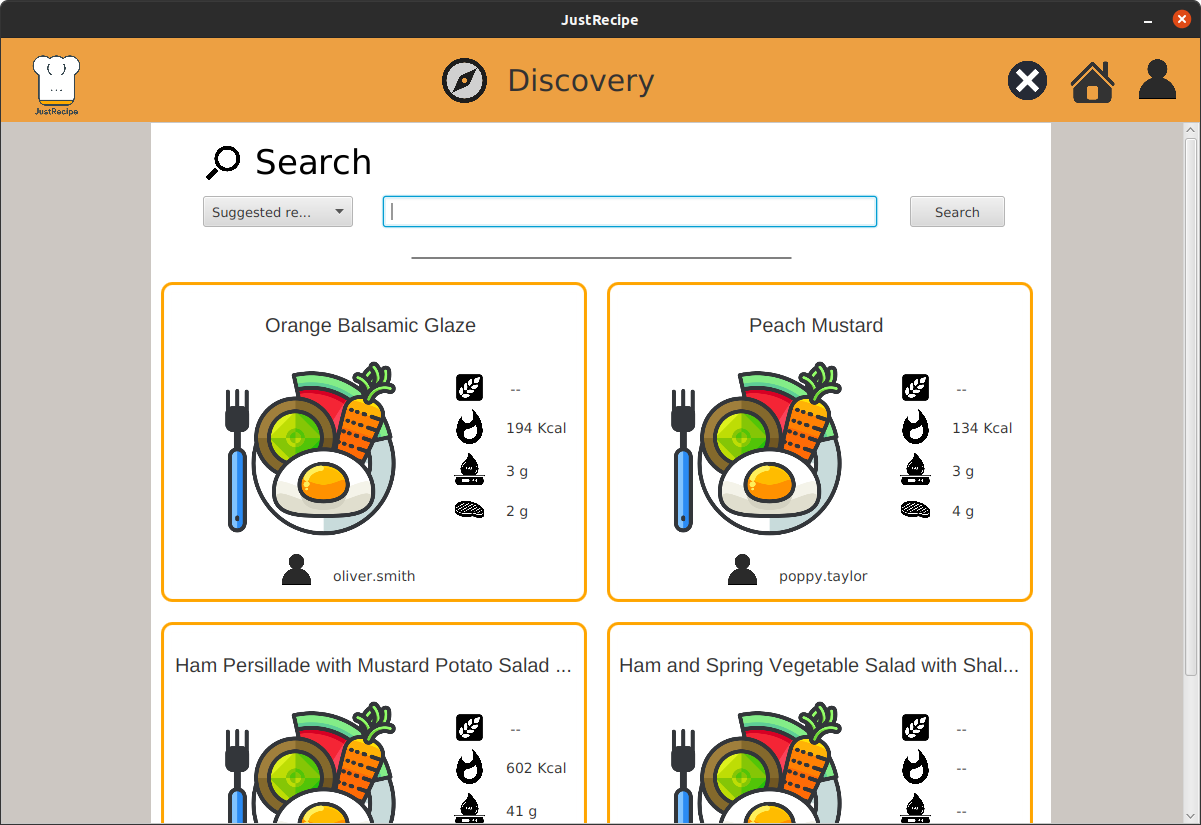
\includegraphics[scale=0.25]{img/user_manual/first-discovery.png}
	\caption{Discovery Page First Access}
\end{figure}

%\newpage
\noindent If the user wants to see the detail of a recipe he can click on its snapshot, where the snapshot is the one showed in figure 4.7.

\begin{figure}[htpb]
	\centering
	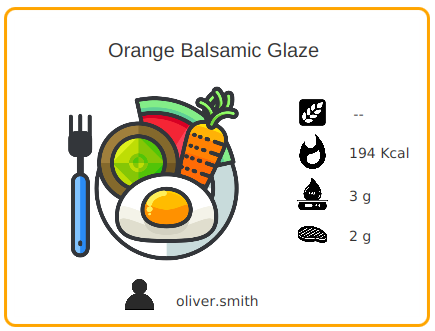
\includegraphics[scale=0.35]{img/user_manual/snap.png}
	\caption{Example of a snapshot}
\end{figure}

\noindent If he clicks on the snapshot the recipe page will be showed, as we can see in figure 4.8.

\begin{figure}[htpb]
	\centering
	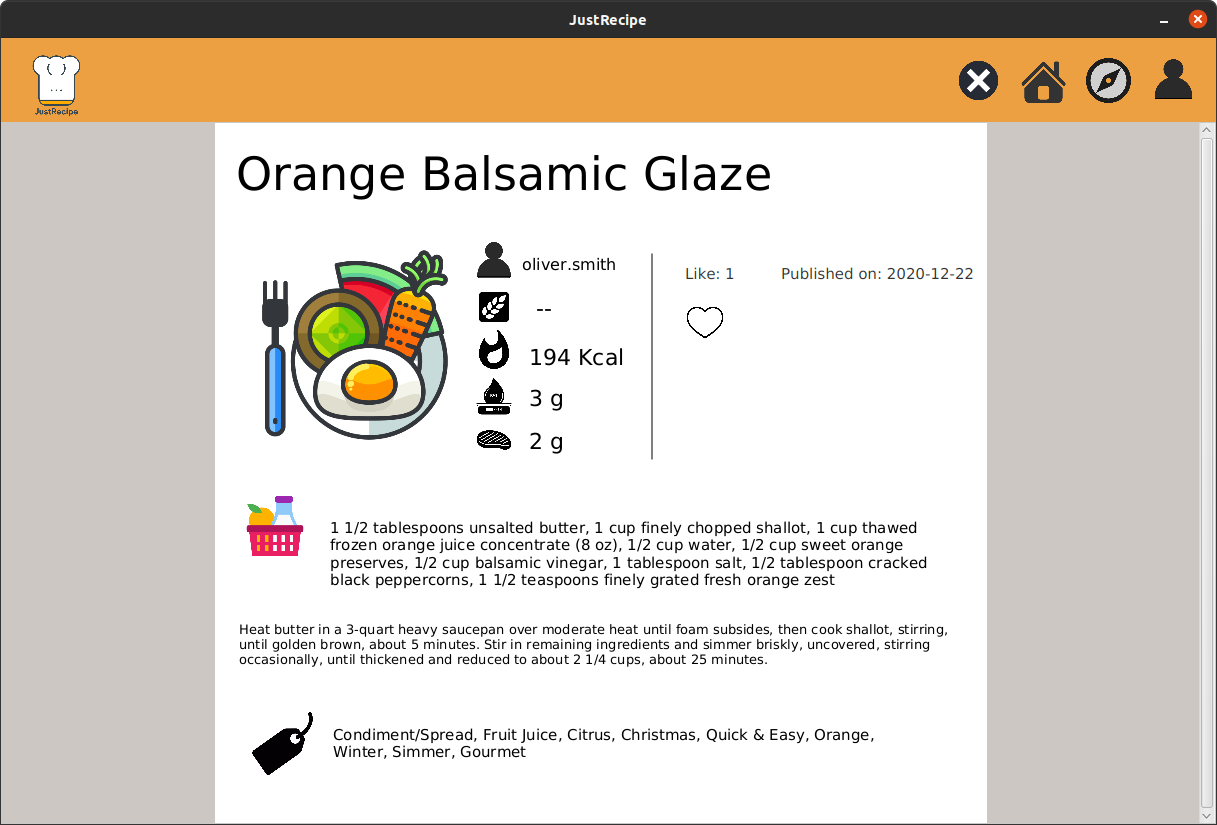
\includegraphics[scale=0.35]{img/user_manual/recipepage.png}
	\caption{Recipe page}
\end{figure}

\noindent Here near the image we can see in order: the username of who has added the recipe, carbs, calories, fat, protein. In the right part we can see how many likes the recipe has, when it was added and then there is the icon that allow us to like the recipe.

\noindent If the user clicks on the heart-like icon, he likes the recipes and the icon will be colored in red in order to show that the logged user has liked this recipe. We can see it in figure 4.9 and 4.10.

\begin{figure}[htpb]
	\centering
	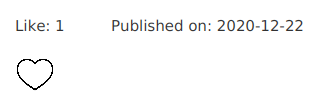
\includegraphics[scale=0.31]{img/user_manual/beforelike.png}
	\caption{Before Like}
\end{figure}


\begin{figure}[htpb]
	\centering
	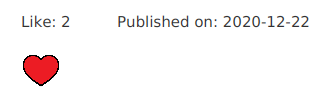
\includegraphics[scale=0.31]{img/user_manual/afterlike.png}
	\caption{After Like}
\end{figure}

\newpage


\noindent Another possibility is that I can follow the user that has added this recipes, in order to do this I must access to his profile page, so I have to click on the user icon or on the user's name as is shown in figure 4.11.

\begin{figure}[htpb]
	\centering
	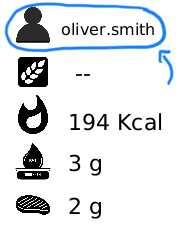
\includegraphics[scale=0.38]{img/user_manual/user-icon.png}
	\caption{User Icon}
\end{figure}

\noindent Then the user page will be shown as we can see in figure 4.12.

\begin{figure}[htpb]
	\centering
	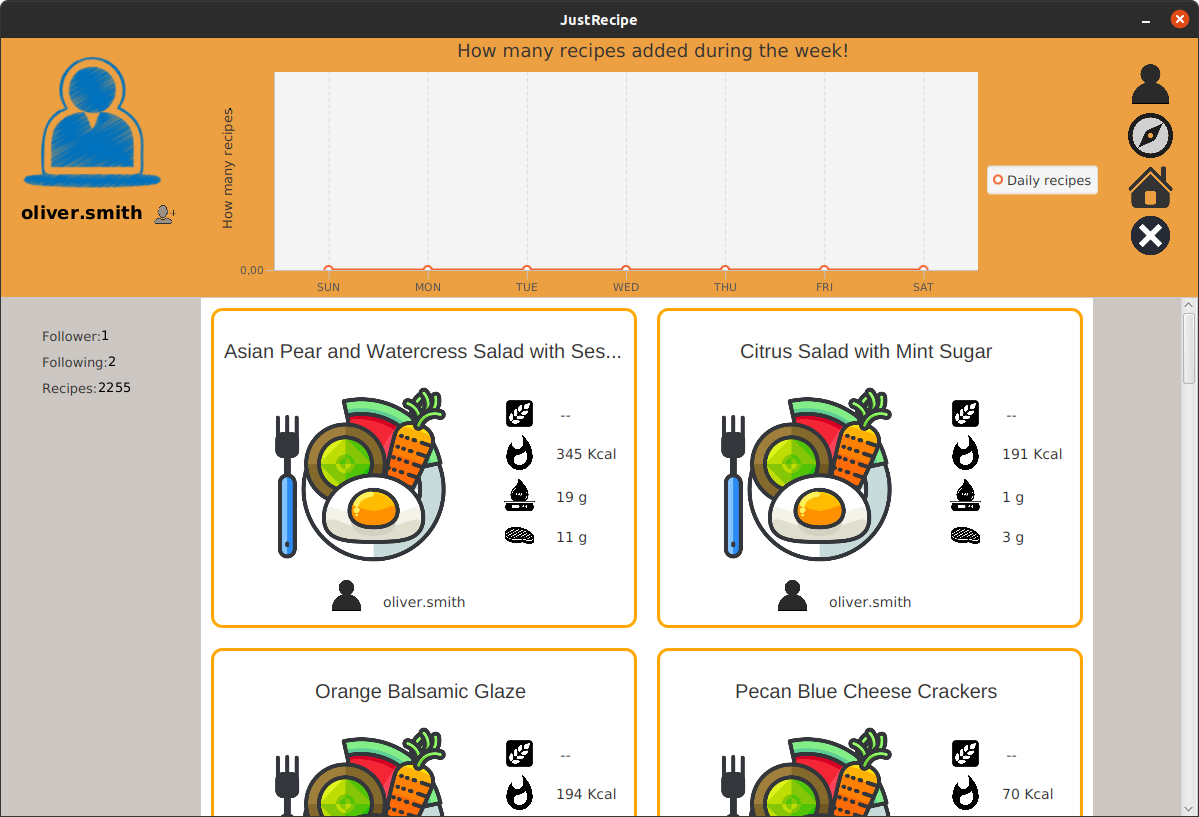
\includegraphics[scale=0.38]{img/user_manual/generic-user-page.png}
	\caption{User Page}
\end{figure}

\noindent If the user wants to follow this user he can click on the correspondent icon near the name of the user as is shown in figure 4.13. After the click the icon changes in order to notify that the logged user has started to follow this user.

\begin{figure}[htpb]
	\centering
	
\includegraphics[scale=0.35]{img/user_manual/howToFollow.png}
	\caption{Before Follow}
\end{figure}

\begin{figure}[htpb]
	\centering
	
\includegraphics[scale=0.35]{img/user_manual/afterfollow.png}
	\caption{After follow}
\end{figure}

\newpage
\noindent Now if we go back to the homepage we will see the recipes added by \emph{oliver.smith} because we follow him. So we can click on the home-like icon and go to the homepage as it is shown in the figure 4.15 and 4.16.

\noindent Only the first 20 recipes are shown, so if we scroll until the end we can click on the button \textbf{Next} to see the next 20, and then the button \textbf{Previous} to see the previous 20. We can see this in figure 4.17 and 4.18.


\begin{figure}[htpb]
	\centering
	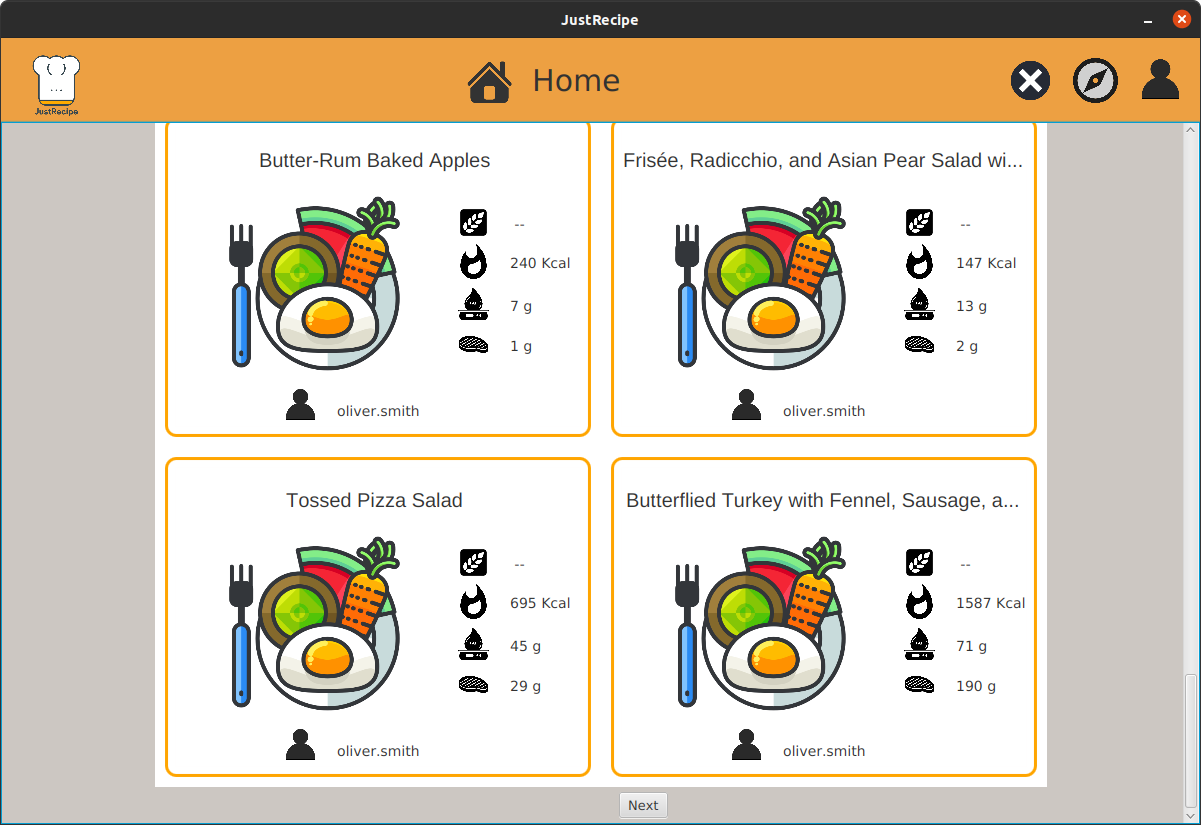
\includegraphics[scale=0.37]{img/user_manual/nextbutton.png}
	\caption{Next Button}
\end{figure}

\begin{figure}[htpb]
	\centering
	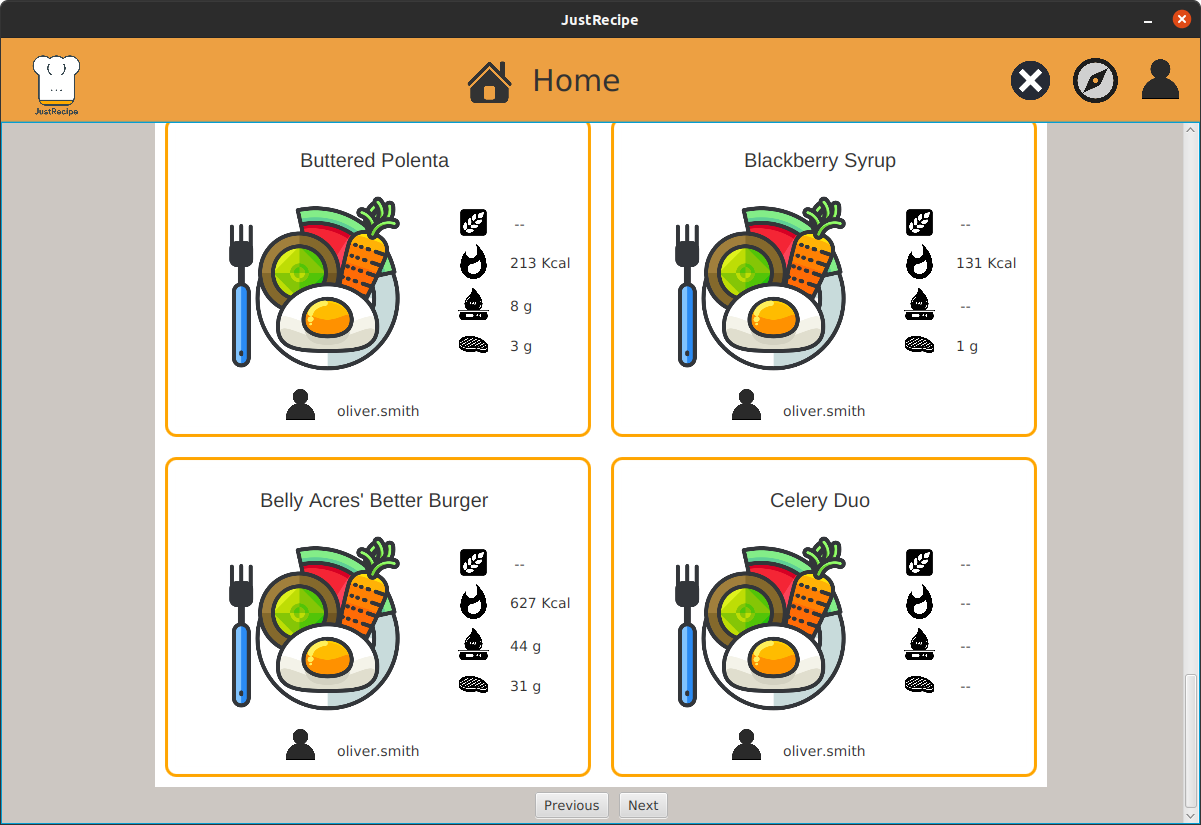
\includegraphics[scale=0.37]{img/user_manual/previousbutton.png}
	\caption{Previous Button}
\end{figure}

\newpage
\section{User Profile}

\end{document}
